% !TeX root = er.tex

\chapter{Processamento de imagem}\label{ch.image}

O sensor de distância em seu carro que dirige sozinho detecta um objeto a $100$ metros na frente do seu carro. Você está seguindo o carro à sua frente a uma distância segura ou tem um pedestre saltando para a estrada? Os algoritmos robóticos apresentados até agora têm sido baseados na medição de propriedades físicas como distância, ângulos e reflectância. Tarefas mais complexas exigem que um robô obtenha informações detalhadas sobre seu ambiente, especialmente quando o robô se destina a funcionar de forma autônoma em um ambiente não familiar.

Para nós, a forma óbvia de fazer sentido ao nosso ambiente é usar a visão. Tomamos a visão como certa e não nos damos conta de quão complexo nosso sistema visual - nossos olhos e cérebro - realmente é. De fato, cerca de $30\%$ do cérebro é usado para a visão. Podemos distinguir instantaneamente entre um carro em movimento e um pedestre atravessando a estrada e reagindo rapidamente.

Por quase duzentos anos foi possível gravar imagens automaticamente usando uma câmera, mas a interpretação das imagens continuou sendo uma tarefa para os humanos. Com o advento dos computadores, tornou-se possível processar e interpretar as imagens automaticamente. As imagens digitais são familiares: mapas meteorológicos de satélites, imagens médicas (raios X, tomografias e ressonâncias magnéticas, imagens de ultra-som) e as fotos que tiramos com nossos smartphones. O campo de \emph{digital image processing} é um dos campos mais intensamente estudados da ciência da computação e engenharia, mas os sistemas de processamento de imagens ainda não atingiram a capacidade do sistema visual humano.

Neste capítulo, apresentamos um gosto dos algoritmos para processamento digital de imagens e descrevemos como eles são usados em sistemas robóticos. As seções~\ref{s.obtaining-images}--\ref{s.image-overview} fornecem uma visão geral dos sistemas de processamento de imagem e processamento de imagem digital. As seções~\ref{s.enhance}--\ref{s.blob} descrevem algoritmos para processamento de imagem: aprimoramento por filtros digitais e manipulação de histograma, segmentação (detecção de bordas) e reconhecimento de características (detecção de cantos e blobs, identificação de múltiplas características).

Por razões de custo e poder computacional, poucos robôs educacionais usam câmeras, portanto, para estudar algoritmos de processamento de imagem é possível implementar os algoritmos em um computador pessoal usando imagens capturadas com uma câmera digital. No entanto, propomos algumas atividades que demonstram algoritmos de processamento de imagem em um robô educacional. O robô se move sobre uma imagem unidimensional e as amostras são lidas por um sensor de terra. Isto resulta em uma matriz unidimensional de pixels que pode ser processada usando versões simplificadas dos algoritmos que apresentamos.

\section{Obtenção de imagens}\label{s.obtaining-images}

Nesta seção, damos uma visão geral das considerações de projeto para sistemas de imagem.

\subsection*{Óptica}

O sistema óptico de uma câmera consiste em uma lente que focaliza a luz em um sensor. Quanto mais larga a lente, mais luz pode ser coletada, o que é importante para sistemas que precisam trabalhar em ambientes escuros. Quanto maior a distância focal (que está relacionada à distância entre a lente e o sensor), maior é a ampliação. É por isso que os fotógrafos profissionais carregam câmeras pesadas com lentes longas. Os fabricantes de smartphones se deparam com um dilema: queremos que nossos telefones sejam finos e elegantes, mas isso limita a distância focal da câmera. Para a maioria das aplicações robóticas, a ampliação não vale o tamanho e o peso necessários para alcançar uma distância focal longa.

\subsection*{Resolução}

Era uma vez, as imagens eram capturadas no filme por uma reação química causada por uma luz atingindo uma folha de plástico coberta com uma emulsão de minúsculas partículas de prata. Em princípio, cada partícula podia reagir independentemente, de modo que a resolução era extremamente alta. Em imagens digitais, a luz é capturada por dispositivos semicondutores, tais como \emph{dispositivos acoplados à carga (CCD)}. Uma câmera digital contém um chip com um número fixo de elementos em uma matriz retangular. Cada elemento mede a intensidade da luz independentemente e estas medidas são chamadas \emph{pixels}. Quanto mais pixels forem capturados por um chip de uma determinada área, maior será a resolução. Atualmente, mesmo câmeras baratas em smartphones podem capturar milhões de pixels em uma única imagem.

O problema das imagens de alta resolução é a grande quantidade de memória necessária para armazená-las. Considere uma tela de computador de alta resolução com $1920\times 1080$ pixels e assuma que cada pixel usa $8$ bits para armazenar intensidade na faixa de $0$--$255$. Uma única imagem requer cerca de $2$ megabytes (MB) de memória. Um computador incorporado poderia analisar uma única imagem desse tipo, mas um robô móvel pode precisar armazenar várias imagens por segundo.

Ainda mais importante do que a quantidade de memória necessária é o poder computacional necessário para analisar as imagens. Os algoritmos de processamento de imagens exigem que o computador faça um cálculo em cada pixel individual. Isto não é um problema para um astrônomo que analisa imagens enviadas à Terra a partir de um telescópio espacial, mas é um problema para um carro que se auto dirige e que precisa tomar decisões em uma fração de segundo.

\subsection*{Cor}

Nosso sistema visual tem a capacidade de distinguir uma gama de comprimentos de onda chamada \emph{visible light}. Distinguimos comprimentos de onda diferentes como cores diferentes. A luz de comprimentos de onda mais longos é chamada \emph{red}, enquanto a luz de comprimentos de onda mais curtos é chamada \emph{violet}. O olho humano pode distinguir milhões de cores diferentes, apesar de nomearmos apenas algumas: vermelho, laranja, amarelo, verde, ciano, azul, violeta, etc. A cor é uma das principais ferramentas que usamos para identificar objetos.

Os sensores são capazes de medir a luz de comprimentos de onda fora do alcance que chamamos de luz visual: luz \emph{infravermelha} de comprimentos de onda mais longos e luz \emph{ultravioleta} de comprimentos de onda mais curtos. As imagens infravermelhas são importantes na robótica porque objetos quentes como pessoas e carros podem ser detectados como luz infravermelha brilhante.

O problema com a cor é que ela triplica os requisitos para o armazenamento e processamento de imagens. Todas as cores podem ser formadas tomando quantidades variáveis das três \emph{primárias cores}: vermelho, verde e azul (RGB). Portanto, uma imagem colorida requer três bytes para cada pixel. Uma única imagem colorida de resolução de $1920\times 1080$ requer mais de $6$ MB de memória para ser armazenada e o processamento da imagem leva pelo menos três vezes mais tempo.

\section[processamento de imagens digitais]{Uma visão geral do processamento de imagens digitais}\label{s.image-overview}

O sistema óptico de um robô captura imagens como matrizes retangulares de pixels, mas as tarefas de um robô são expressas em termos de objetos do ambiente: entrar em uma sala através de uma porta, pegar um item de uma prateleira, parar se um pedestre caminhar na frente do carro. Como podemos passar de pixels a objetos?

A primeira etapa é \emph{image enhancement}. As imagens contêm ruídos que resultam da ótica e da eletrônica. Além disso, a iluminação do ambiente pode fazer com que uma imagem fique muito escura ou lavada; a imagem pode ser girada acidentalmente; a imagem pode estar desfocada. Todos estes problemas são independentes do conteúdo. Não importa se uma imagem que esteja fora de foco mostra um gato ou uma criança. Os algoritmos de melhoria de imagem normalmente funcionam modificando os valores atribuídos a pixels individuais sem considerar seu significado.\footnote{Nós nos limitamos a algoritmos de processamento \emph{espacial} que funcionam nos próprios pixels. Há outra abordagem chamada \emph{freqüência} processing algorithms, mas que requer técnicas matemáticas além do escopo deste livro.}

A melhoria da imagem é difícil porque não há uma definição formal do que significa melhorar uma imagem. Uma mancha embaçada pode ser sujeira nas lentes de uma câmera ou em uma galáxia desconhecida. A seção~\ref{s.enhance} apresenta duas abordagens para melhorar a imagem: a filtragem remove o ruído ao substituir um pixel por uma média de seus pixels vizinhos e a manipulação do histograma modifica o brilho e o contraste de uma imagem.

Os objetos são distinguidos por linhas, curvas e áreas. Uma porta consiste em três bordas retas de um retângulo com um lado curto em falta. Um semáforo consiste em três discos brilhantes, um acima do outro. Antes que uma porta ou semáforo possa ser identificado, os algoritmos de processamento de imagem devem determinar quais pixels representam linhas, bordas, etc. Este processo é chamado \emph{segmentação} ou \emph{extração de características} porque os algoritmos têm que determinar quais pixels fazem parte de um segmento de uma imagem.

A segmentação seria fácil se as bordas, linhas e curvas fossem uniformes, mas isto não é o que ocorre em imagens reais. Uma borda pode ser inclinada em um ângulo arbitrário e alguns de seus pixels podem estar obscurecidos por sombras ou até mesmo ausentes. Estamos familiarizados com \emph{captchas} onde as letras são intencionalmente distorcidas para tornar o reconhecimento automático muito difícil, enquanto que os humanos podem facilmente identificar letras distorcidas. Algoritmos de melhoria podem facilitar a segmentação, por exemplo, ao preencher os pixels faltantes, mas também podem introduzir segmentos artificiais. A seção~\ref{s.edge-detection} demonstra uma técnica de segmentação: um filtro que detecta bordas em uma imagem.

A fase final do processamento da imagem é o reconhecimento de objetos. Em Sect.~\ref{s.corners}, apresentamos dois algoritmos de detecção de cantos: pela localização da interseção de duas bordas e pela contagem de vizinhos com intensidades semelhantes. A seção~\ref{s.blob} descreve como reconhecer \emph{blobs}, que são áreas cujos pixels têm intensidades semelhantes, mas que não são delimitadas por características regulares, como linhas e curvas. Finalmente, Activity~\ref{act.recognize} demonstra o reconhecimento de um objeto que é definido por mais de uma característica, tal como uma porta definida por duas arestas que estão a uma distância arbitrária uma da outra.

\section{Melhoria de imagem}\label{s.enhance}

A figura~\ref{fig.no-noise} mostra uma imagem de um retângulo cuja intensidade é uniforme horizontalmente e sombreada de cima para baixo de escuro à luz. A representação da imagem como uma matriz retangular de pixels de $6,00\times 10$ é mostrada na Fig.~\ref{fig.pixel-noise}, onde cada pixel é representado por um nível de intensidade de luz na faixa de $0$--$100$. Agora veja a Fig.~\ref{fig.noise}: a imagem não é mais \emph{smooth} no sentido de que há três pontos cuja intensidade não é similar às intensidades de seus vizinhos. Compare a matriz de pixels na Fig.~\ref{fig.pixel-noise} com a da Fig.~\ref{fig.pixel-noise}: as intensidades dos pixels nos locais $(2,3)$, $(3,6)$, $(4,4)$ são diferentes. Isto é provavelmente o resultado de ruído e não uma característica real do objeto que está sendo fotografado. 

\begin{figure}
\begin{minipage}{.45\textwidth}

\begin{tikzpicture}
\shade[bottom color=black!40,top color=black!80] (0,0) rectangle +(4,1);
\end{tikzpicture}
\caption{Imagem sem ruído}\label{fig.no-noise}
\end{minipage}
\hspace{\fill}
\begin{minipage}{.45\textwidth}

\begin{tikzpicture}
\shade[bottom color=black!40,top color=black!80] (0,0) rectangle +(4,1);
\draw[fill,color=black!70] ( 8mm,5mm) rectangle +(1mm,1mm);
\draw[fill,color=black!80] (30mm,3mm) rectangle +(1mm,1mm);
\draw[fill,color=black!20] (15mm,2mm) rectangle +(1mm,1mm);
\end{tikzpicture}
\caption{Imagem com ruído}\label{fig.noise}
\end{minipage}
\end{figure}

%\begin{figure}
%\subfigures
%\begin{minipage}{\textwidth}
%\leftfigure{
%\begin{tikzpicture}
%\shade[bottom color=black!40,top color=black!80] (0,0) rectangle +(4,1);
%\end{tikzpicture}
%}
%\hspace{\fill}
%\rightfigure{
%\begin{tikzpicture}
%\shade[bottom color=black!40,top color=black!80] (0,0) rectangle +(4,1);
%\draw[fill,color=black!70] ( 8mm,5mm) rectangle +(1mm,1mm);
%\draw[fill,color=black!80] (30mm,3mm) rectangle +(1mm,1mm);
%\draw[fill,color=black!20] (15mm,2mm) rectangle +(1mm,1mm);
%\end{tikzpicture}
%}
%\leftcaption{Image without noise}\label{fig.no-noise}
%\rightcaption{Image with noise}\label{fig.noise}
%\end{minipage}
%\end{figure}

\begin{figure}
\begin{minipage}{.5\textwidth}
\begin{tabular}{r@{\hspace{4pt}}r@{\hspace{4pt}}r@{\hspace{4pt}}r@{\hspace{4pt}}r@{\hspace{4pt}}r@{\hspace{4pt}}r@{\hspace{4pt}}r@{\hspace{4pt}}r@{\hspace{4pt}}r@{\hspace{4pt}}r}
& $\scriptstyle 0$ & $\scriptstyle 1$ & $\scriptstyle 2$ & $\scriptstyle 3$ & $\scriptstyle 4$ & $\scriptstyle 5$ & $\scriptstyle 6$ & $\scriptstyle 7$ & $\scriptstyle 8$ & $\scriptstyle 9$ \\
$\scriptstyle 0$ & $10$ & $10$ & $10$ & $10$ & 	$10$ & $10$ & $10$ & $10$ & $10$ & $10$\\
$\scriptstyle 1$ & $20$ & $20$ & $20$ & $20$ & $20$ & $20$ & $20$ & $20$ & $20$ & $20$\\
$\scriptstyle 2$ & $30$ & $30$ & $30$ & $30$ & $30$ & $30$ & $30$ & $30$ & $30$ & $30$\\
$\scriptstyle 3$ & $40$ & $40$ & $40$ & $40$ & $40$ & $40$ & $40$ & $40$ & $40$ & $40$\\                   
$\scriptstyle 4$ & $50$ & $50$ & $50$ & $50$ & $50$ & $50$ & $50$ & $50$ & $50$ & $50$\\
$\scriptstyle 5$ & $60$ & $60$ & $60$ & $60$ & $60$ & $60$ & $60$ & $60$ & $60$ & $60$\\
\end{tabular}
\caption{Conjunto de pixel sem ruído}\label{fig.pixel-no-noise}
\end{minipage}
\hspace{\fill}
\begin{minipage}{.5\textwidth}
\begin{tabular}{r@{\hspace{4pt}}r@{\hspace{4pt}}r@{\hspace{4pt}}r@{\hspace{4pt}}r@{\hspace{4pt}}r@{\hspace{4pt}}r@{\hspace{4pt}}r@{\hspace{4pt}}r@{\hspace{4pt}}r@{\hspace{4pt}}r}
& $\scriptstyle 0$ & $\scriptstyle 1$ & $\scriptstyle 2$ & $\scriptstyle 3$ & $\scriptstyle 4$ & $\scriptstyle 5$ & $\scriptstyle 6$ & $\scriptstyle 7$ & $\scriptstyle 8$ & $\scriptstyle 9$ \\
$\scriptstyle 0$ & $10$ & $10$ & $10$ & $10$ & $10$ & $10$ & $10$ & $10$ & $10$ & $10$\\
$\scriptstyle 1$ & $20$ & $20$ & $20$ & $20$ & $20$ & $20$ & $20$ & $20$ & $20$ & $20$\\
$\scriptstyle 2$ & $30$ & $30$ & $30$ & \boldmath $20$ & $30$ & $30$ & $30$ & $30$ & $30$ & $30$\\
$\scriptstyle 3$ & $40$ & $40$ & $40$ & $40$ & $40$ & $40$ & \boldmath $10$ & $40$ & $40$ & $40$\\
$\scriptstyle 4$ & $50$ & $50$ & $50$ & $50$ & \boldmath $90$ & $50$ & $50$ & $50$ & $50$ & $50$\\
$\scriptstyle 5$ & $60$ & $60$ & $60$ & $60$ & $60$ & $60$ & $60$ & $60$ & $60$ & $60$\\
\end{tabular}
\caption{Conjunto de pixel com ruído}\label{fig.pixel-noise}
\end{minipage}
\end{figure}

%\begin{figure}
%\subfigures
%\begin{minipage}{\textwidth}
%\leftfigure{
%\begin{tabular}{r@{\hspace{4pt}}r@{\hspace{6pt}}r@{\hspace{6pt}}r@{\hspace{6pt}}r@{\hspace{6pt}}r@{\hspace{6pt}}r@{\hspace{6pt}}r@{\hspace{6pt}}r@{\hspace{6pt}}r@{\hspace{6pt}}r}
%& $\scriptstyle 0$ & $\scriptstyle 1$ & $\scriptstyle 2$ & $\scriptstyle 3$ & $\scriptstyle 4$ & $\scriptstyle 5$ & $\scriptstyle 6$ & $\scriptstyle 7$ & $\scriptstyle 8$ & $\scriptstyle 9$ \\
%$\scriptstyle 0$ & $10$ & $10$ & $10$ & $10$ & 	$10$ & $10$ & $10$ & $10$ & $10$ & $10$\\
%$\scriptstyle 1$ & $20$ & $20$ & $20$ & $20$ & $20$ & $20$ & $20$ & $20$ & $20$ & $20$\\
%$\scriptstyle 2$ & $30$ & $30$ & $30$ & $30$ & $30$ & $30$ & $30$ & $30$ & $30$ & $30$\\
%$\scriptstyle 3$ & $40$ & $40$ & $40$ & $40$ & $40$ & $40$ & $40$ & $40$ & $40$ & $40$\\                   
%$\scriptstyle 4$ & $50$ & $50$ & $50$ & $50$ & $50$ & $50$ & $50$ & $50$ & $50$ & $50$\\
%$\scriptstyle 5$ & $60$ & $60$ & $60$ & $60$ & $60$ & $60$ & $60$ & $60$ & $60$ & $60$\\
%\end{tabular}
%}
%\hspace{\fill}
%\rightfigure{
%\begin{tabular}{r@{\hspace{4pt}}r@{\hspace{6pt}}r@{\hspace{6pt}}r@{\hspace{6pt}}r@{\hspace{6pt}}r@{\hspace{6pt}}r@{\hspace{6pt}}r@{\hspace{6pt}}r@{\hspace{6pt}}r@{\hspace{6pt}}r}
%& $\scriptstyle 0$ & $\scriptstyle 1$ & $\scriptstyle 2$ & $\scriptstyle 3$ & $\scriptstyle 4$ & $\scriptstyle 5$ & $\scriptstyle 6$ & $\scriptstyle 7$ & $\scriptstyle 8$ & $\scriptstyle 9$ \\
%$\scriptstyle 0$ & $10$ & $10$ & $10$ & $10$ & $10$ & $10$ & $10$ & $10$ & $10$ & $10$\\
%$\scriptstyle 1$ & $20$ & $20$ & $20$ & $20$ & $20$ & $20$ & $20$ & $20$ & $20$ & $20$\\
%$\scriptstyle 2$ & $30$ & $30$ & $30$ & \boldmath $20$ & $30$ & $30$ & $30$ & $30$ & $30$ & $30$\\
%$\scriptstyle 3$ & $40$ & $40$ & $40$ & $40$ & $40$ & $40$ & \boldmath $10$ & $40$ & $40$ & $40$\\
%$\scriptstyle 4$ & $50$ & $50$ & $50$ & $50$ & \boldmath $90$ & $50$ & $50$ & $50$ & $50$ & $50$\\
%$\scriptstyle 5$ & $60$ & $60$ & $60$ & $60$ & $60$ & $60$ & $60$ & $60$ & $60$ & $60$\\
%\end{tabular}
%}
%\leftcaption{Pixel array without noise}\label{fig.pixel-no-noise}
%\rightcaption{Pixel array with noise}\label{fig.pixel-noise}
%\end{minipage}
%\end{figure}

Não importa realmente de onde vem o ruído: do próprio objeto, poeira na lente da câmera, não-uniformidade no sensor ou ruído na eletrônica. É impossível nos livrarmos inteiramente do ruído, porque nunca podemos ter certeza se um pixel é ruído ou uma característica real do objeto, mas queremos melhorar a imagem para que o ruído não seja mais perceptível.

\subsection{Spatial filters}

Considere a linha $4$ na matriz de pixels em Fig.~\ref{fig.pixel-noise}:
\[
50,\, 50,\, 50,\,50,\, 90,\, 50,\, 50,\, 50,\, 50,\, 50\,.
\]
Figura~\ref{fig.before-average} é um gráfico da intensidade da luz $f$ para os pixels naquela linha. É claro que um dos pixels tem um valor improvável porque seu valor é muito diferente do de seus vizinhos. Um programa pode tornar cada pixel mais parecido com seus vizinhos, substituindo a intensidade do pixel pela média de sua intensidade e as intensidades de seus vizinhos. Para a maioria dos pixels da linha, isto não muda seus valores: $(50+50+50)/3=50$, mas o pixel de ruído e seus dois vizinhos recebem novos valores: $(50+90+50)/3\approx 60$ (Fig.~\ref{fig.after-average}). A média fez com que dois pixels recebessem valores "errados", mas em geral a imagem será visualmente melhorada porque a intensidade do ruído será reduzida.

\begin{figure}
\begin{minipage}{.47\textwidth}
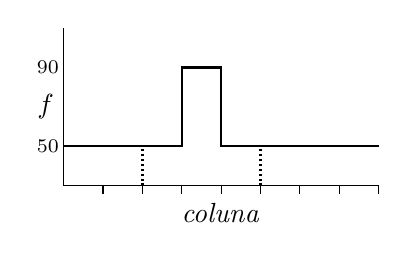
\begin{tikzpicture}[scale=1]
\draw (0,2) -- node[left] {$f$} (0,0) -- node[below,yshift=-1mm] {\textit{coluna}} (4,0);
\draw[thick] (0,.5) -- (1.5,.5) -- (1.5,1.5) -- (2,1.5) -- (2,.5) -- (4,.5);
\node at (-2mm,.5) {$\scriptstyle 50$};
\node at (-2mm,1.5) {$\scriptstyle 90$};
\foreach \x in {.5,1,1.5,2,2.5,3,3.5,4}
  \draw[thin] (\x,-1mm) -- (\x,0);
\draw[densely dotted,thick] (1,0) -- (1,.5);
\draw[densely dotted,thick] (2.5,0) -- (2.5,.5);
\end{tikzpicture}
\caption{Gráfico de intensidade antes de fazer a média}\label{fig.before-average}
\end{minipage}
\hspace{\fill}
\begin{minipage}{.47\textwidth}
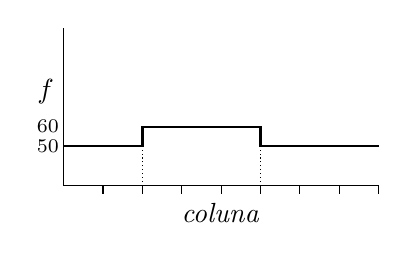
\begin{tikzpicture}[scale=1]
\draw (0,2) -- node[left,yshift=2mm] {$f$} (0,0) -- node[below,yshift=-1mm] {\textit{coluna}} (4,0);
\draw[thick] (0,.5) -- (1,.5) -- (1,.75) -- (2.5,.75) -- (2.5,.5) -- (4,.5);
\node at (-2mm,.5) {$\scriptstyle 50$};
\node at (-2mm,.75) {$\scriptstyle 60$};
\foreach \x in {.5,1,1.5,2,2.5,3,3.5,4}
  \draw[thin] (\x,-1mm) -- (\x,0);
\draw[densely dotted] (1,0) -- (1,.5);
\draw[densely dotted] (2.5,0) -- (2.5,.5);
\end{tikzpicture}
\caption{Gráfico de Intensidade após o cálculo da média}\label{fig.after-average}
\end{minipage}
\end{figure}

%\begin{figure}
%\subfigures
%\begin{minipage}{\textwidth}
%\leftfigure{
%\begin{tikzpicture}[scale=1.2]
%\draw (0,2) -- node[left] {$f$} (0,0) -- node[below,yshift=-1mm] {\textit{column}} (4,0);
%\draw[thick] (0,.5) -- (1.5,.5) -- (1.5,1.5) -- (2,1.5) -- (2,.5) -- (4,.5);
%\node at (-2mm,.5) {$\scriptstyle 50$};
%\node at (-2mm,1.5) {$\scriptstyle 90$};
%\foreach \x in {.5,1,1.5,2,2.5,3,3.5,4}
%  \draw[thin] (\x,-1mm) -- (\x,0);
%\draw[densely dotted,thick] (1,0) -- (1,.5);
%\draw[densely dotted,thick] (2.5,0) -- (2.5,.5);
%\end{tikzpicture}
%}
%\hspace{\fill}
%\rightfigure{
%\begin{tikzpicture}[scale=1.2]
%\draw (0,2) -- node[left,yshift=2mm] {$f$} (0,0) -- node[below,yshift=-1mm] {\textit{column}} (4,0);
%\draw[thick] (0,.5) -- (1,.5) -- (1,.75) -- (2.5,.75) -- (2.5,.5) -- (4,.5);
%\node at (-2mm,.5) {$\scriptstyle 50$};
%\node at (-2mm,.75) {$\scriptstyle 60$};
%\foreach \x in {.5,1,1.5,2,2.5,3,3.5,4}
%  \draw[thin] (\x,-1mm) -- (\x,0);
%\draw[densely dotted] (1,0) -- (1,.5);
%\draw[densely dotted] (2.5,0) -- (2.5,.5);
%\end{tikzpicture}
%}
%\leftcaption{Intensity plot before averaging}\label{fig.before-average}
%\rightcaption{Intensity plot after averaging}\label{fig.after-average}
%\end{minipage}
%\end{figure}

Tomando a média de uma seqüência de pixels é a versão discreta da integração de uma função de intensidade contínua. A integração suaviza a variação local da função. As linhas pontilhadas nas Figs.~\ref{fig.before-average}--\ref{fig.after-average} indicam uma seqüência de três pixels e pode-se ver que as áreas delimitadas são mais ou menos as mesmas.

A operação de média é realizada aplicando um filtro de espaço em cada pixel da imagem.\footnote{O termo matemático para aplicar uma função $g$ em cada ponto de uma função $f$ é chamado de (discreto) \emph{convolução}. Para funções contínuas, a integração é usada no lugar da adição de média.} Para a matriz bidimensional de pixels, o filtro é representado por uma matriz de $3\times 3$, onde cada elemento da matriz especifica o fator pelo qual o pixel e seus vizinhos são multiplicados. Cada pixel tem quatro ou oito vizinhos, dependendo se incluímos os vizinhos diagonais. Aqui, incluímos os píxeis diagonais nos filtros.

O \emph{filtro da caixa} é:
\[
\left[
\begin{array}{ccc}
1 & 1 & 1\\
1 & 1 & 1\\
1 & 1 & 1
\end{array}
\right]\,.
\]
Os resultados das multiplicações são adicionados e a soma é dividida por $9$ para redimensionar o resultado para um valor de intensidade.

A aplicação do filtro a cada pixel $(r,c)$ pode ser escrita explicitamente como:
\[
\begin{array}{llll}
g(r,c) = &(\\
&f(r-1,c-1) & \;+\; f(r-1,c) & \;+\; f(r-1,c+1) \;+\\
&f(r,c-1) & \;+\; f(r,c) & \;+\; f(r,c+1) \;\;\;\;\;\;\;+\\
&f(r+1,c-1) & \;+\; f(r+1,c) & \;+\; f(r+1,c+1)\\
& ) \; / \; 9\,.
\end{array}
\]
O resultado da aplicação do filtro de caixa à imagem ruidosa na Fig.~\ref{fig.pixel-noise} é mostrado na Fig.~\ref{fig.box-filter}.\footnote{O filtro não é aplicado aos pixels no limite da imagem para evitar exceder os limites da matriz. Alternativamente, a imagem pode ser acolchoada com filas e colunas extras.} Os valores de intensidade não são mais uniformes, mas estão bastante próximos dos valores originais, exceto quando havia um pixel de ruído. A segunda linha do fundo mostra que o valor do ruído de $90$ não aparece mais; em vez disso, todos os valores na linha estão próximos uns dos outros na faixa $46$--$54$.

\begin{figure}
\begin{minipage}{.5\textwidth}
\begin{tabular}{r@{\hspace{4pt}}r@{\hspace{4pt}}r@{\hspace{4pt}}r@{\hspace{4pt}}r@{\hspace{4pt}}r@{\hspace{4pt}}r@{\hspace{4pt}}r@{\hspace{4pt}}r@{\hspace{4pt}}r@{\hspace{4pt}}r}
& $\scriptstyle 0$ & $\scriptstyle 1$ & $\scriptstyle 2$ & $\scriptstyle 3$ & $\scriptstyle 4$ & $\scriptstyle 5$ & $\scriptstyle 6$ & $\scriptstyle 7$ & $\scriptstyle 8$ & $\scriptstyle 9$ \\
$\scriptstyle 0$ & 10 & 10 & 10 & 10 & 10 & 10 & 10 & 10 & 10 & 10\\
$\scriptstyle 1$ & 20 & 20 & 18 & 18 & 18 & 20 & 20 & 20 & 20 & 20\\
$\scriptstyle 2$ & 30 & 30 & 28 & 28 & 28 & 26 & 26 & 26 & 30 & 30\\
$\scriptstyle 3$ & 40 & 40 & 38 & 43 & 43 & 41 & 36 & 36 & 40 & 40\\
$\scriptstyle 4$ & 50 & 50 & 50 & 54 & 54 & 51 & 46 & 46 & 50 & 50\\
$\scriptstyle 5$ & 60 & 60 & 60 & 60 & 60 & 60 & 60 & 60 & 60 & 60\\
\end{tabular}
\caption{Sde alisamento com o filtro da caixa}\label{fig.box-filter}
\end{minipage}
\hspace{\fill}
\begin{minipage}{.5\textwidth}
\begin{tabular}{r@{\hspace{4pt}}r@{\hspace{4pt}}r@{\hspace{4pt}}r@{\hspace{4pt}}r@{\hspace{4pt}}r@{\hspace{4pt}}r@{\hspace{4pt}}r@{\hspace{4pt}}r@{\hspace{4pt}}r@{\hspace{4pt}}r}
& $\scriptstyle 0$ & $\scriptstyle 1$ & $\scriptstyle 2$ & $\scriptstyle 3$ & $\scriptstyle 4$ & $\scriptstyle 5$ & $\scriptstyle 6$ & $\scriptstyle 7$ & $\scriptstyle 8$ & $\scriptstyle 9$ \\
$\scriptstyle 0$ & 10 & 10 & 10 & 10 & 10 & 10 & 10 & 10 & 10 & 10\\
$\scriptstyle 1$ & 20 & 20 & 19 & 19 & 19 & 20 & 20 & 20 & 20 & 20\\
$\scriptstyle 2$ & 30 & 30 & 29 & 25 & 29 & 28 & 28 & 28 & 30 & 30\\
$\scriptstyle 3$ & 40 & 40 & 39 & 41 & 41 & 40 & 25 & 38 & 40 & 40\\
$\scriptstyle 4$ & 50 & 50 & 50 & 52 & 70 & 50 & 48 & 48 & 50 & 50\\
$\scriptstyle 5$ & 60 & 60 & 60 & 60 & 60 & 60 & 60 & 60 & 60 & 60\\
\end{tabular}
\caption{Alisamento com um filtro ponderado}\label{fig.weighted-filter}
\end{minipage}
\end{figure}


%\begin{figure}
%\subfigures
%\begin{minipage}{\textwidth}
%\leftfigure{
%\begin{tabular}{r@{\hspace{4pt}}r@{\hspace{6pt}}r@{\hspace{6pt}}r@{\hspace{6pt}}r@{\hspace{6pt}}r@{\hspace{6pt}}r@{\hspace{6pt}}r@{\hspace{6pt}}r@{\hspace{6pt}}r@{\hspace{6pt}}r}
%& $\scriptstyle 0$ & $\scriptstyle 1$ & $\scriptstyle 2$ & $\scriptstyle 3$ & $\scriptstyle 4$ & $\scriptstyle 5$ & $\scriptstyle 6$ & $\scriptstyle 7$ & $\scriptstyle 8$ & $\scriptstyle 9$ \\
%$\scriptstyle 0$ & 10 & 10 & 10 & 10 & 10 & 10 & 10 & 10 & 10 & 10\\
%$\scriptstyle 1$ & 20 & 20 & 18 & 18 & 18 & 20 & 20 & 20 & 20 & 20\\
%$\scriptstyle 2$ & 30 & 30 & 28 & 28 & 28 & 26 & 26 & 26 & 30 & 30\\
%$\scriptstyle 3$ & 40 & 40 & 38 & 43 & 43 & 41 & 36 & 36 & 40 & 40\\
%$\scriptstyle 4$ & 50 & 50 & 50 & 54 & 54 & 51 & 46 & 46 & 50 & 50\\
%$\scriptstyle 5$ & 60 & 60 & 60 & 60 & 60 & 60 & 60 & 60 & 60 & 60\\
%\end{tabular}
%}
%\hspace{\fill}
%\rightfigure{
%\begin{tabular}{r@{\hspace{4pt}}r@{\hspace{6pt}}r@{\hspace{6pt}}r@{\hspace{6pt}}r@{\hspace{6pt}}r@{\hspace{6pt}}r@{\hspace{6pt}}r@{\hspace{6pt}}r@{\hspace{6pt}}r@{\hspace{6pt}}r}
%& $\scriptstyle 0$ & $\scriptstyle 1$ & $\scriptstyle 2$ & $\scriptstyle 3$ & $\scriptstyle 4$ & $\scriptstyle 5$ & $\scriptstyle 6$ & $\scriptstyle 7$ & $\scriptstyle 8$ & $\scriptstyle 9$ \\
%$\scriptstyle 0$ & 10 & 10 & 10 & 10 & 10 & 10 & 10 & 10 & 10 & 10\\
%$\scriptstyle 1$ & 20 & 20 & 19 & 19 & 19 & 20 & 20 & 20 & 20 & 20\\
%$\scriptstyle 2$ & 30 & 30 & 29 & 25 & 29 & 28 & 28 & 28 & 30 & 30\\
%$\scriptstyle 3$ & 40 & 40 & 39 & 41 & 41 & 40 & 25 & 38 & 40 & 40\\
%$\scriptstyle 4$ & 50 & 50 & 50 & 52 & 70 & 50 & 48 & 48 & 50 & 50\\
%$\scriptstyle 5$ & 60 & 60 & 60 & 60 & 60 & 60 & 60 & 60 & 60 & 60\\
%\end{tabular}
%}
%\leftcaption{Smoothing with the box filter}\label{fig.box-filter}
%\rightcaption{Smoothing with a weighted filter}\label{fig.weighted-filter}
%\end{minipage}
%\end{figure}

O filtro da caixa dá igual importância ao pixel e a todos os seus vizinhos, mas um filtro \emph{pesado} utiliza diferentes fatores para diferentes pixels. O seguinte filtro dá muito mais peso ao próprio pixel do que a seus vizinhos:
\[
\left[
\begin{array}{ccc}
1 & 1 & 1\\
1 & 8 & 1\\
1 & 1 & 1
\end{array}
\right]\,.
\]
Seria apropriado usar este filtro se pensarmos que um pixel quase certamente tem seu valor correto, mas ainda queremos que seus vizinhos influenciem seu valor. Após a aplicação deste filtro, o resultado deve ser dividido por $16$ para escalar a soma a um valor de intensidade. A figura~\ref{fig.weighted-filter} mostra o resultado da utilização do filtro ponderado. Olhando novamente para a segunda linha do fundo, o valor de $90$ só foi reduzido para $70$ porque é dado maior peso ao pixel em relação a seus vizinhos.

\begin{framed}
\act{Melhoria de imagem: suavização}{smoothing}
\begin{itemize}
\item Imprimir uma folha de papel com um padrão de nível de cinza como o mostrado na Fig.~\ref{fig.one-enhance}. O padrão tem duas linhas pretas que desejamos detectar, mas também três áreas cinza-escuras (indicadas pelas setas) que provavelmente serão detectadas incorretamente como linhas.
\item Programar o robô de modo que ele se mova da esquerda para a direita sobre o padrão, amostrando a saída do sensor de terra. Examine a saída e defina um limite para que o robô detecte tanto as linhas pretas quanto as áreas de cinza escuro. Modifique o programa para que em sua segunda passagem, indique (por luz ou som) quando tiver detectado uma linha preta e uma área escura.
\item Modificar o programa para que ele substitua cada amostra pela média da intensidade da amostra e de seus dois vizinhos. O robô deve agora detectar as duas linhas pretas, mas não as áreas cinzentas.
\item Experimentar com pesos diferentes para a média.
\item Experimento com diferentes taxas de amostragem. O que acontece se o sensor do solo for amostrado em intervalos muito curtos?
\end{itemize}
\end{framed}

\begin{figure}
\begin{center}
\begin{tikzpicture}
\pic at (-2,1.5) { robot };
\draw[fill,gray] (-1,1.3) rectangle +(6pt,12pt);
\foreach \n/\colorb/\colort in
  {-.5/40/50, 0/50/70, .5/70/40, 1/40/50, 1.5/50/70, 2.0/70/50, 2.5/50/40,%
   4/40/50, 4.5/50/70, 5/70/50, 5.5/50/40,%
   7/40/50, 7.5/50/40, 8/40/40}
    \shade[left color=black!\colorb,right color=black!\colort] (\n,0) rectangle +(5mm,3);
\foreach \x in {.5,2,5}
  \draw[->] (\x, -.4) -- (\x, -.1);
\draw[fill,color=black] (3,0) rectangle +(1,3);
\draw[fill,color=black] (6,0) rectangle +(1,3);
\end{tikzpicture}
\caption{Melhoria de imagem unidimensional}\label{fig.one-enhance}
\end{center}
\end{figure}

\subsection{Manipulação de histogramas}

A figura~\ref{fig.binary-noise} mostra os pixels de uma imagem binária: uma imagem onde cada pixel é preto ou branco.\footnote{Os valores $10$ para preto e $90$ para branco foram usados ao invés dos mais usuais $0$ e $100$ para clareza na impressão da matriz.} Timagem mostra um retângulo branco de $3\times 5$ sobre o fundo preto. A figura~\ref{fig.binary-noise} mostra a mesma imagem com muito ruído aleatório adicionado. Olhando para a imagem é possível identificar o retângulo, mas é muito difícil de fazer e suavizar a imagem não ajudará.

\begin{figure}
\begin{minipage}{.5\textwidth}
\begin{tabular}{r@{\hspace{4pt}}r@{\hspace{4pt}}r@{\hspace{4pt}}r@{\hspace{4pt}}r@{\hspace{4pt}}r@{\hspace{4pt}}r@{\hspace{4pt}}r@{\hspace{4pt}}r@{\hspace{4pt}}r@{\hspace{4pt}}r}
& $\scriptstyle 0$ & $\scriptstyle 1$ & $\scriptstyle 2$ & $\scriptstyle 3$ & $\scriptstyle 4$ & $\scriptstyle 5$ & $\scriptstyle 6$ & $\scriptstyle 7$ & $\scriptstyle 8$ & $\scriptstyle 9$ \\
$\scriptstyle 0$ & $10$ & $10$ & $10$ & $10$ & $10$ & $10$ & $10$ & $10$ & $10$ & $10$\\
$\scriptstyle 1$ & $10$ & $10$ & $10$ & $10$ & $10$ & $10$ & $10$ & $10$ & $10$ & $10$\\
$\scriptstyle 2$ & $10$ & $10$ & $10$ & \boldmath $90$ & \boldmath $90$ & \boldmath $90$ & \boldmath $90$ & \boldmath $90$ & $10$ & $10$\\
$\scriptstyle 3$ & $10$ & $10$ & $10$ & \boldmath $90$ & \boldmath $90$ & \boldmath $90$ & \boldmath $90$ & \boldmath $90$ & $10$ & $10$\\
$\scriptstyle 4$ & $10$ & $10$ & $10$ & \boldmath $90$ & \boldmath $90$ & \boldmath $90$ & \boldmath $90$ & \boldmath $90$ & $10$ & $10$\\
$\scriptstyle 5$ & $10$ & $10$ & $10$ & $10$ & $10$ & $10$ & $10$ & $10$ & $10$ & $10$\\
\end{tabular}
\caption{Imagem binária sem ruído}\label{fig.binary-no-noise}\end{minipage}
\hspace{\fill}
\begin{minipage}{.5\textwidth}
\begin{tabular}{r@{\hspace{4pt}}r@{\hspace{4pt}}r@{\hspace{4pt}}r@{\hspace{4pt}}r@{\hspace{4pt}}r@{\hspace{4pt}}r@{\hspace{4pt}}r@{\hspace{4pt}}r@{\hspace{4pt}}r@{\hspace{4pt}}r}
& $\scriptstyle 0$ & $\scriptstyle 1$ & $\scriptstyle 2$ & $\scriptstyle 3$ & $\scriptstyle 4$ & $\scriptstyle 5$ & $\scriptstyle 6$ & $\scriptstyle 7$ & $\scriptstyle 8$ & $\scriptstyle 9$ \\
$\scriptstyle 0$ & $19$ & $17$ & $37$ & $19$ & $26$ & $11$ & $46$ & $27$ & $37$ & $10$\\
$\scriptstyle 1$ & $11$ & $24$ & $17$ & $30$ & $14$ & $43$ & $29$ & $22$ & $34$ & $46$\\
$\scriptstyle 2$ & $31$ & $37$ & $38$ & $63$ & $72$ & $86$ & $65$ & $64$ & $27$ & $47$\\
$\scriptstyle 3$ & $33$ & $38$ & $49$ & $73$ & $63$ & $66$ & $59$ & $76$ & $40$ & $10$\\
$\scriptstyle 4$ & $47$ & $13$ & $44$ & $90$ & $86$ & $56$ & $63$ & $65$ & $18$ & $44$\\
$\scriptstyle 5$ & $10$ & $34$ & $29$ & $14$ & $35$ & $31$ & $26$ & $42$ & $15$ & $25$\\
\end{tabular}
\caption{Imagem binária com ruído}\label{fig.binary-noise}
\end{minipage}
\end{figure}

%\begin{figure}
%\subfigures
%\begin{minipage}{\textwidth}
%\leftfigure{
%\begin{tabular}{r@{\hspace{4pt}}r@{\hspace{6pt}}r@{\hspace{6pt}}r@{\hspace{6pt}}r@{\hspace{6pt}}r@{\hspace{6pt}}r@{\hspace{6pt}}r@{\hspace{6pt}}r@{\hspace{6pt}}r@{\hspace{6pt}}r}
%& $\scriptstyle 0$ & $\scriptstyle 1$ & $\scriptstyle 2$ & $\scriptstyle 3$ & $\scriptstyle 4$ & $\scriptstyle 5$ & $\scriptstyle 6$ & $\scriptstyle 7$ & $\scriptstyle 8$ & $\scriptstyle 9$ \\
%$\scriptstyle 0$ & $10$ & $10$ & $10$ & $10$ & $10$ & $10$ & $10$ & $10$ & $10$ & $10$\\
%$\scriptstyle 1$ & $10$ & $10$ & $10$ & $10$ & $10$ & $10$ & $10$ & $10$ & $10$ & $10$\\
%$\scriptstyle 2$ & $10$ & $10$ & $10$ & \boldmath $90$ & \boldmath $90$ & \boldmath $90$ & \boldmath $90$ & \boldmath $90$ & $10$ & $10$\\
%$\scriptstyle 3$ & $10$ & $10$ & $10$ & \boldmath $90$ & \boldmath $90$ & \boldmath $90$ & \boldmath $90$ & \boldmath $90$ & $10$ & $10$\\
%$\scriptstyle 4$ & $10$ & $10$ & $10$ & \boldmath $90$ & \boldmath $90$ & \boldmath $90$ & \boldmath $90$ & \boldmath $90$ & $10$ & $10$\\
%$\scriptstyle 5$ & $10$ & $10$ & $10$ & $10$ & $10$ & $10$ & $10$ & $10$ & $10$ & $10$\\
%\end{tabular}
%}
%\hspace{\fill}
%\rightfigure{
%\begin{tabular}{r@{\hspace{4pt}}r@{\hspace{6pt}}r@{\hspace{6pt}}r@{\hspace{6pt}}r@{\hspace{6pt}}r@{\hspace{6pt}}r@{\hspace{6pt}}r@{\hspace{6pt}}r@{\hspace{6pt}}r@{\hspace{6pt}}r}
%& $\scriptstyle 0$ & $\scriptstyle 1$ & $\scriptstyle 2$ & $\scriptstyle 3$ & $\scriptstyle 4$ & $\scriptstyle 5$ & $\scriptstyle 6$ & $\scriptstyle 7$ & $\scriptstyle 8$ & $\scriptstyle 9$ \\
%$\scriptstyle 0$ & $19$ & $17$ & $37$ & $19$ & $26$ & $11$ & $46$ & $27$ & $37$ & $10$\\
%$\scriptstyle 1$ & $11$ & $24$ & $17$ & $30$ & $14$ & $43$ & $29$ & $22$ & $34$ & $46$\\
%$\scriptstyle 2$ & $31$ & $37$ & $38$ & $63$ & $72$ & $86$ & $65$ & $64$ & $27$ & $47$\\
%$\scriptstyle 3$ & $33$ & $38$ & $49$ & $73$ & $63$ & $66$ & $59$ & $76$ & $40$ & $10$\\
%$\scriptstyle 4$ & $47$ & $13$ & $44$ & $90$ & $86$ & $56$ & $63$ & $65$ & $18$ & $44$\\
%$\scriptstyle 5$ & $10$ & $34$ & $29$ & $14$ & $35$ & $31$ & $26$ & $42$ & $15$ & $25$\\
%\end{tabular}
%}
%\leftcaption{Binary image without noise}\label{fig.binary-no-noise}
%\rightcaption{Binary image with noise}\label{fig.binary-noise}
%\end{minipage}
%\end{figure}

Vamos agora construir um \emph{histograma} das intensidades (Fig.~\ref{fig.hist}). Um histograma é construído de \emph{silos}, onde cada contentor armazena uma contagem dos pixels com uma gama de intensidades. O histograma na figura contém dez caixas para intensidades nas faixas de $0$--$9$, $10$--$19$, \ldots, $91$--$99$. Se assumirmos que o retângulo branco é pequeno em relação ao fundo, é fácil ver pelo histograma que existem dois grupos de pixels, aqueles que são relativamente escuros e aqueles que são relativamente brilhantes. Um limiar de $50$ ou $60$ deve ser capaz de distinguir entre o retângulo e o fundo, mesmo na presença de ruído. De fato, um limiar de $50$ restaura a imagem original, enquanto um limiar de $60$ restaura corretamente $13$ dos $15$ pixels do retângulo.

\begin{figure}
\begin{center}
\begin{tikzpicture}
\draw (0,2) -- node[left,xshift=-2mm] {\textit{contar}} (0,0) -- node[below,yshift=-5mm] {\textit{intensidade}} (10,0);
\foreach \n/\v/\y/\lab in {0/0/0/0--9, 1/14/1.4/10--19, 2/9/.9/20--29, 3/12/1.2/30--39, 4/10/1/40--49, 5/2/.2/50--59, 6/7/.7/60--69, 7/3/.3/70--79, 8/2/.2/80--89, 9/1/.1/90--99}
  \pic { barhist=\n/\v/\y/\lab };
\end{tikzpicture}
\caption{Histograma da imagem ruidosa}\label{fig.hist}
\end{center}
\end{figure}

A vantagem da manipulação de histogramas é que é muito eficiente computar até mesmo em imagens grandes. Para cada pixel, divida a intensidade pelo número de caixas e aumente o número de caixas:
\begin{quote}
\p{for each pixel p}\\
\hspace*{2em}\p{bin\_number} $\leftarrow$ \p{intensity(p) / number\_of\_bins}\\
\hspace*{2em}\p{bins[bin\_number]} $\leftarrow$ \p{bins[bin\_number] + 1}
\end{quote}
Compare esta operação com a aplicação de um $3\times 3$ filtro espacial que requer multiplicações de $9$, adições de $8$ e uma divisão em cada pixel. Além disso, é necessária pouca memória. Escolhemos caixas de $10$ para que Fig.~\ref{fig.hist} pudesse exibir todo o histograma, mas um histograma completo de $8$-bits em escala de cinza requer apenas caixas de $256$.

Escolher um limiar examinando uma trama do histograma é fácil, e se você souber aproximadamente a fração de fundo coberta pelos objetos, a seleção do limiar pode ser feita automaticamente.

Algoritmos para manipulação do histograma podem realizar melhorias mais complexas do que o simples limiar binário que descrevemos aqui. Em particular, existem algoritmos para melhorar imagens modificando o brilho e o contraste de uma imagem. 

\begin{framed}
\act{Melhoria de imagem: manipulação de histograma}{hist}
\begin{itemize}
\item Modificar o programa em Activity~\ref{act.smoothing} para que ele calcule o histograma das amostras.
\item Como o histograma muda se o número de amostras é aumentado?
\item Examine o histograma para determinar um limiar que será usado para distinguir entre as linhas pretas e o fundo.
\item Calcule a soma do conteúdo das caixas até que a soma seja maior que uma fração (talvez um terço) das amostras. Use o índice da última lixeira para definir o limite.
\end{itemize}
\end{framed}

\section{Detecção de bordas}\label{s.edge-detection}

Os sistemas de processamento de imagem médica precisam de algoritmos sofisticados de melhoria de imagem para modificar o brilho e o contraste, remover ruídos, etc. Entretanto, uma vez que a imagem é aprimorada, a interpretação da imagem é feita por especialistas que sabem quais linhas e sombras correspondem a quais órgãos do corpo, e se os órgãos são normais ou não. Um robô autônomo não tem um humano para fazer interpretação: ele precisa identificar objetos como portas em um prédio, caixas em um armazém e carros na estrada. O primeiro passo é extrair características ou segmentos, tais como linhas, bordas e áreas.

\begin{figure}
\begin{minipage}{.5\textwidth}
\begin{tabular}{r@{\hspace{4pt}}r@{\hspace{6pt}}r@{\hspace{6pt}}r@{\hspace{6pt}}r@{\hspace{6pt}}r@{\hspace{6pt}}r@{\hspace{6pt}}r@{\hspace{6pt}}r@{\hspace{6pt}}r@{\hspace{6pt}}r}
& $\scriptstyle 0$ & $\scriptstyle 1$ & $\scriptstyle 2$ & $\scriptstyle 3$ & $\scriptstyle 4$ & $\scriptstyle 5$\\
$\scriptstyle 0$ & $30$ & $30$ & $30$ & $30$ & $30$ &$30$\\
$\scriptstyle 1$ & $30$ & $30$ & $30$ & $30$ & $30$ &$30$\\
$\scriptstyle 2$ & $30$ & $30$ & $30$ & $30$ & $30$ &$30$\\
$\scriptstyle 3$ & \boldmath $50$ & \boldmath $50$ & \boldmath $50$ & \boldmath $50$ & \boldmath $50$ & \boldmath $50$\\
$\scriptstyle 4$ & \boldmath $50$ & \boldmath $50$ & \boldmath $50$ & \boldmath $50$ & \boldmath $50$ & \boldmath $50$\\
$\scriptstyle 5$ & \boldmath $50$ & \boldmath $50$ & \boldmath $50$ & \boldmath $50$ & \boldmath $50$ & \boldmath $50$\\
\end{tabular}
\caption{Imagem com uma borda}\label{fig.edge}
\end{minipage}
\hspace{\fill}
\begin{minipage}{.5\textwidth}
\begin{tikzpicture}[scale=1.5,baseline=-18mm]
\draw (0,1) -- node[left] {$f$} (0,0) -- node[below,yshift=-2mm] {\textit{linha}} (3,0);
\draw[thick] (0,.25) -- (1.5,.25) -- (2,.75) -- (3,.75);
\node at (-1.5mm,.2) {\scriptsize{30}};
\node at (-1.5mm,.8) {\scriptsize{50}};
\foreach \x in {.5,1,1.5,2,2.5,3}
  \draw[thin] (\x,-1mm) -- (\x,0);
\end{tikzpicture}
\caption{Intensidade da borda}\label{fig.edge-intensity}
\end{minipage}
\end{figure}

%\begin{figure}
%\subfigures
%\begin{minipage}{\textwidth}
%\leftfigure{
%\begin{tabular}{r@{\hspace{4pt}}r@{\hspace{6pt}}r@{\hspace{6pt}}r@{\hspace{6pt}}r@{\hspace{6pt}}r@{\hspace{6pt}}r@{\hspace{6pt}}r@{\hspace{6pt}}r@{\hspace{6pt}}r@{\hspace{6pt}}r}
%& $\scriptstyle 0$ & $\scriptstyle 1$ & $\scriptstyle 2$ & $\scriptstyle 3$ & $\scriptstyle 4$ & $\scriptstyle 5$\\
%$\scriptstyle 0$ & $30$ & $30$ & $30$ & $30$ & $30$ &$30$\\
%$\scriptstyle 1$ & $30$ & $30$ & $30$ & $30$ & $30$ &$30$\\
%$\scriptstyle 2$ & $30$ & $30$ & $30$ & $30$ & $30$ &$30$\\
%$\scriptstyle 3$ & \boldmath $50$ & \boldmath $50$ & \boldmath $50$ & \boldmath $50$ & \boldmath $50$ & \boldmath $50$\\
%$\scriptstyle 4$ & \boldmath $50$ & \boldmath $50$ & \boldmath $50$ & \boldmath $50$ & \boldmath $50$ & \boldmath $50$\\
%$\scriptstyle 5$ & \boldmath $50$ & \boldmath $50$ & \boldmath $50$ & \boldmath $50$ & \boldmath $50$ & \boldmath $50$\\
%\end{tabular}
%}
%\hspace{\fill}
%\rightfigure{
%\begin{tikzpicture}[scale=1.7]
%\draw (0,1) -- node[left] {$f$} (0,0) -- node[below,yshift=-2mm] {\textit{row}} (3,0);
%\draw[thick] (0,.25) -- (1.5,.25) -- (2,.75) -- (3,.75);
%\node at (-1.5mm,.2) {\scriptsize{30}};
%\node at (-1.5mm,.8) {\scriptsize{50}};
%\foreach \x in {.5,1,1.5,2,2.5,3}
%  \draw[thin] (\x,-1mm) -- (\x,0);
%\end{tikzpicture}
%}
%\leftcaption{Image with an edge}\label{fig.edge}
%\rightcaption{Intensity of edge}\label{fig.edge-intensity}
%\end{minipage}
%\end{figure}

Considere o conjunto de pixels de $6\times 6$ em Fig.~\ref{fig.edge}. O nível de intensidade de cada linha é uniforme, mas há uma descontinuidade acentuada entre o nível de intensidade das linhas de $2$ e $3$. Claramente, isto representa uma borda entre a área escura na parte superior e a área clara na parte inferior. O cálculo da média tornará a mudança de intensidade mais suave e perderemos a mudança acentuada na borda.

\begin{figure}
\begin{minipage}{.5\textwidth}
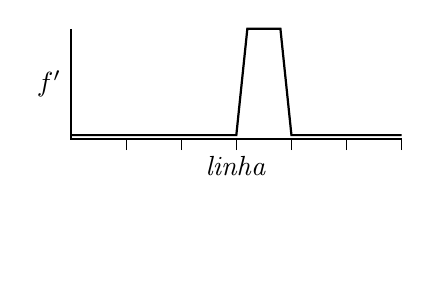
\begin{tikzpicture}[scale=1.4,baseline=-1.5cm]
\draw (0,1) -- node[left] {$f'$} (0,0) -- node[below,yshift=-1mm] {\textit{linha}} (3,0);
\draw[thick] (0,1pt) -- (1.5,1pt) -- (1.6,1) -- (1.9,1) -- (2,1pt) -- (3,1pt);
\foreach \x in {.5,1,1.5,2,2.5,3}
  \draw[thin] (\x,-1mm) -- (\x,0);
\end{tikzpicture}
\caption{Primeira derivada de intensidade de borda}
\label{fig.edge-first}
\end{minipage}
\hspace{\fill}
\begin{minipage}{.5\textwidth}
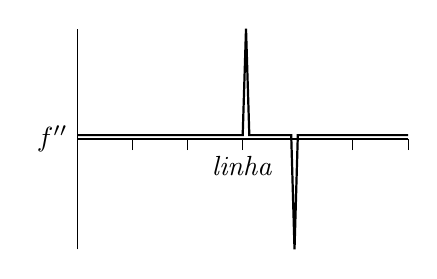
\begin{tikzpicture}[scale=1.4]
\draw (0,-1) -- node[left] {$f''$} (0,1);
\draw (0,0) -- node[below,yshift=-1mm] {\textit{linha}} (3,0);
\draw[thick] (0,1pt) -- (1.5,1pt) -- (1.53,1) -- (1.56,1pt) -- (1.94,1pt) -- (1.97,-1) -- (2,1pt) -- (3,1pt);
\foreach \x in {.5,1,1.5,2,2.5,3}
  \draw[thin] (\x,-1mm) -- (\x,0);
\end{tikzpicture}
\caption{Segunda derivada da intensidade da borda}\label{fig.edge-second}
\end{minipage}
\end{figure}

%\begin{figure}
%\subfigures
%\begin{minipage}{\textwidth}
%\leftfigure{
%\begin{tikzpicture}[scale=1.6,baseline=-1.5cm]
%\draw (0,1) -- node[left] {$f'$} (0,0) -- node[below,yshift=-1mm] {\textit{row}} (3,0);
%\draw[thick] (0,1pt) -- (1.5,1pt) -- (1.6,1) -- (1.9,1) -- (2,1pt) -- (3,1pt);
%\foreach \x in {.5,1,1.5,2,2.5,3}
%  \draw[thin] (\x,-1mm) -- (\x,0);
%\end{tikzpicture}
%}
%\hspace{\fill}
%\rightfigure{
%\begin{tikzpicture}[scale=1.6]
%\draw (0,-1) -- node[left] {$f''$} (0,1);
%\draw (0,0) -- node[below,yshift=-1mm] {\textit{row}} (3,0);
%\draw[thick] (0,1pt) -- (1.5,1pt) -- (1.53,1) -- (1.56,1pt) -- (1.94,1pt) -- (1.97,-1) -- (2,1pt) -- (3,1pt);
%\foreach \x in {.5,1,1.5,2,2.5,3}
%  \draw[thin] (\x,-1mm) -- (\x,0);
%\end{tikzpicture}
%}
%\leftcaption{First derivative of edge intensity}\label{fig.edge-first}
%\rightcaption{Second derivative of edge intensity}\label{fig.edge-second}
%\end{minipage}
%\end{figure}

Como a média é um operador integrador que suprime mudanças abruptas de intensidade, não é surpreendente que o operador diferencial possa ser usado para \emph{detectar} mudanças abruptas que representam bordas. Figura~\ref{fig.edge-intensity} traça a intensidade contra o número da linha ao longo de uma única coluna da Fig.~\ref{fig.edge}, embora as intensidades sejam mostradas como linhas ao invés de pontos discretos. A intensidade não muda para os três primeiros pixels, depois aumenta rapidamente e continua no nível mais alto. A primeira derivada $f'$ de uma função $f$ é zero quando $f$ é constante, positiva quando $f$ aumenta e negativa quando $f$ diminui. Isto é mostrado na Fig.~\ref{fig.edge-first}. Uma borda pode ser detectada pela busca de um rápido aumento ou diminuição da primeira derivada da intensidade da imagem.

Na prática, é melhor usar a segunda derivada. A figura~\ref{fig.edge-second} mostra um gráfico de $f''$, a derivada de $f'$ na fig.~\ref{fig.edge-first}. O pico positivo seguido do pico negativo indica uma transição do escuro para o claro; se a transição fosse do claro para o escuro, o pico negativo precederia o pico positivo.

Existem muitos operadores de derivados digitais. Um simples mas eficaz é o \emph{Sobel filter}. Há dois filtros, um para detectar bordas horizontais (à esquerda) e outro para detectar bordas verticais (à direita):
\[
\begin{array}{c@{\hspace{4em}}c}
\left[
\begin{array}{rrr}
-1 & -2 & -1\\
0 & 0 & 0\\
1 & 2 & 1\\
\end{array}
\right]
&
\left[
\begin{array}{rrr}
-1 & 0 & 1\\
-2 & 0 & 2\\
-1 & 0 & 1\\
\end{array}
\right]\,.
\end{array}
\]
Uma característica de um filtro derivado é que a soma de seus elementos deve ser igual a zero. A razão é que se o operador é aplicado a um pixel cuja intensidade é a mesma de todos os seus vizinhos, o resultado deve ser igual a zero. Veja novamente as Figs.~\ref{fig.edge-intensity} e \ref{fig.edge-first} onde a derivada é zero quando a intensidade é constante.

Quando os filtros Sobel são aplicados à matriz de pixels na Fig.~\ref{fig.edge}, o resultado detecta claramente que existe uma borda horizontal (Fig.~\ref{fig.sobel-horizontal}), mas nenhuma borda vertical (Fig.~\ref{fig.sobel-vertical}).

\begin{figure}
\begin{minipage}{.45\textwidth}
\begin{tabular}{r@{\hspace{4pt}}r@{\hspace{6pt}}r@{\hspace{6pt}}r@{\hspace{6pt}}r@{\hspace{6pt}}r@{\hspace{6pt}}r@{\hspace{6pt}}r@{\hspace{6pt}}r@{\hspace{6pt}}r@{\hspace{6pt}}r}
& $\scriptstyle 0$ & $\scriptstyle 1$ & $\scriptstyle 2$ & $\scriptstyle 3$ & $\scriptstyle 4$ & $\scriptstyle 5$\\
$\scriptstyle 0$ &    $0$ &   $0$ &   $0$ &   $0$ &   $0$ &   $0$ \\
$\scriptstyle 1$ &    $0$ &   $0$ &   $0$ &   $0$ &   $0$ &   $0$ \\
$\scriptstyle 2$ &    $0$ &  $80$ &  $80$ &  $80$ &  $80$ &   $0$ \\
$\scriptstyle 3$ &    $0$ &  $80$ &  $80$ &  $80$ &  $80$ &   $0$ \\
$\scriptstyle 4$ &    $0$ &   $0$ &   $0$ &   $0$ &   $0$ &   $0$ \\
$\scriptstyle 5$ &    $0$ &   $0$ &   $0$ &   $0$ &   $0$ &   $0$ \\
\end{tabular}
\caption{Borda horizontal Sobel}\label{fig.sobel-horizontal}
\end{minipage}
\hspace{\fill}
\begin{minipage}{.45\textwidth}
\begin{tabular}{r@{\hspace{4pt}}r@{\hspace{6pt}}r@{\hspace{6pt}}r@{\hspace{6pt}}r@{\hspace{6pt}}r@{\hspace{6pt}}r@{\hspace{6pt}}r@{\hspace{6pt}}r@{\hspace{6pt}}r@{\hspace{6pt}}r}
& $\scriptstyle 0$ & $\scriptstyle 1$ & $\scriptstyle 2$ & $\scriptstyle 3$ & $\scriptstyle 4$ & $\scriptstyle 5$\\
$\scriptstyle 0$ &    $0$ &   $0$ &   $0$ &   $0$ &   $0$ &   $0$ \\
$\scriptstyle 1$ &    $0$ &   $0$ &   $0$ &   $0$ &   $0$ &   $0$ \\
$\scriptstyle 2$ &    $0$ &   $0$ &   $0$ &   $0$ &   $0$ &   $0$ \\
$\scriptstyle 3$ &    $0$ &   $0$ &   $0$ &   $0$ &   $0$ &   $0$ \\
$\scriptstyle 4$ &    $0$ &   $0$ &   $0$ &   $0$ &   $0$ &   $0$ \\
$\scriptstyle 5$ &    $0$ &   $0$ &   $0$ &   $0$ &   $0$ &   $0$ \\
\end{tabular}
\caption{Borda vertical Sobel}\label{fig.sobel-vertical}
\end{minipage}
\end{figure}


%\begin{figure}
%\subfigures
%\begin{minipage}{\textwidth}
%\leftfigure{
%\begin{tabular}{r@{\hspace{4pt}}r@{\hspace{6pt}}r@{\hspace{6pt}}r@{\hspace{6pt}}r@{\hspace{6pt}}r@{\hspace{6pt}}r@{\hspace{6pt}}r@{\hspace{6pt}}r@{\hspace{6pt}}r@{\hspace{6pt}}r}
%& $\scriptstyle 0$ & $\scriptstyle 1$ & $\scriptstyle 2$ & $\scriptstyle 3$ & $\scriptstyle 4$ & $\scriptstyle 5$\\
%$\scriptstyle 0$ &    $0$ &   $0$ &   $0$ &   $0$ &   $0$ &   $0$ \\
%$\scriptstyle 1$ &    $0$ &   $0$ &   $0$ &   $0$ &   $0$ &   $0$ \\
%$\scriptstyle 2$ &    $0$ &  $80$ &  $80$ &  $80$ &  $80$ &   $0$ \\
%$\scriptstyle 3$ &    $0$ &  $80$ &  $80$ &  $80$ &  $80$ &   $0$ \\
%$\scriptstyle 4$ &    $0$ &   $0$ &   $0$ &   $0$ &   $0$ &   $0$ \\
%$\scriptstyle 5$ &    $0$ &   $0$ &   $0$ &   $0$ &   $0$ &   $0$ \\
%\end{tabular}
%}
%\hspace{\fill}
%\rightfigure{
%\begin{tabular}{r@{\hspace{4pt}}r@{\hspace{6pt}}r@{\hspace{6pt}}r@{\hspace{6pt}}r@{\hspace{6pt}}r@{\hspace{6pt}}r@{\hspace{6pt}}r@{\hspace{6pt}}r@{\hspace{6pt}}r@{\hspace{6pt}}r}
%& $\scriptstyle 0$ & $\scriptstyle 1$ & $\scriptstyle 2$ & $\scriptstyle 3$ & $\scriptstyle 4$ & $\scriptstyle 5$\\
%$\scriptstyle 0$ &    $0$ &   $0$ &   $0$ &   $0$ &   $0$ &   $0$ \\
%$\scriptstyle 1$ &    $0$ &   $0$ &   $0$ &   $0$ &   $0$ &   $0$ \\
%$\scriptstyle 2$ &    $0$ &   $0$ &   $0$ &   $0$ &   $0$ &   $0$ \\
%$\scriptstyle 3$ &    $0$ &   $0$ &   $0$ &   $0$ &   $0$ &   $0$ \\
%$\scriptstyle 4$ &    $0$ &   $0$ &   $0$ &   $0$ &   $0$ &   $0$ \\
%$\scriptstyle 5$ &    $0$ &   $0$ &   $0$ &   $0$ &   $0$ &   $0$ \\
%\end{tabular}
%}
%\leftcaption{Sobel horizontal edge}\label{fig.sobel-horizontal}
%\rightcaption{Sobel vertical edge}\label{fig.sobel-vertical}
%\end{minipage}
%\end{figure}

Os filtros Sobel são muito potentes porque podem não apenas detectar uma borda, mas também calcular o ângulo da borda dentro da imagem. A figura~\ref{fig.diagonal-edge} mostra uma imagem com uma borda correndo diagonalmente da parte superior esquerda para a parte inferior direita. Os resultados da aplicação dos dois filtros Sobel são mostrados nas Figs.~\ref{fig.sobel-diagonal-horizontal}--\ref{fig.sobel-diagonal-vertical}. A partir das magnitudes e sinais dos elementos destas matrizes, o ângulo da borda pode ser computado como descrito em \cite[Sect.~4.3.1]{siegwart}.

\begin{figure}
\begin{tabular}{r@{\hspace{4pt}}r@{\hspace{6pt}}r@{\hspace{6pt}}r@{\hspace{6pt}}r@{\hspace{6pt}}r@{\hspace{6pt}}r@{\hspace{6pt}}r@{\hspace{6pt}}r@{\hspace{6pt}}r@{\hspace{6pt}}r}
& $\scriptstyle 0$ & $\scriptstyle 1$ & $\scriptstyle 2$ & $\scriptstyle 3$ & $\scriptstyle 4$ & $\scriptstyle 5$\\
$\scriptstyle 0$ &    $30$ &   $30$ &   $30$ &   $30$ &   $30$ & $30$ \\
$\scriptstyle 1$ &    \boldmath $50$ &   $30$ &   $30$ &   $30$ &   $30$ & $30$ \\
$\scriptstyle 2$ &    \boldmath $50$ &   \boldmath 50$$ &   $30$ &   $30$ &   $30$ & $30$ \\
$\scriptstyle 3$ &    \boldmath $50$ &   \boldmath $50$ &   \boldmath $50$ &   $30$ &   $30$ & $30$ \\
$\scriptstyle 4$ &    \boldmath $50$ &   \boldmath $50$ &   \boldmath $50$ &   \boldmath $50$ &   $30$ & $30$ \\
$\scriptstyle 5$ &    \boldmath $50$ &   \boldmath $50$ &   \boldmath $50$ &   \boldmath $50$ &   \boldmath $50$ & $30$ \\
\end{tabular}
\caption{Borda diagonal}\label{fig.diagonal-edge}
\end{figure}

\begin{figure}
\begin{minipage}{.45\textwidth}
\begin{tabular}{r@{\hspace{4pt}}r@{\hspace{6pt}}r@{\hspace{6pt}}r@{\hspace{6pt}}r@{\hspace{6pt}}r@{\hspace{6pt}}r@{\hspace{6pt}}r@{\hspace{6pt}}r@{\hspace{6pt}}r@{\hspace{6pt}}r}
& $\scriptstyle 0$ & $\scriptstyle 1$ & $\scriptstyle 2$ & $\scriptstyle 3$ & $\scriptstyle 4$ & $\scriptstyle 5$\\
$\scriptstyle 0$ &    $0$ &   $0$ &   $0$ &   $0$ &   $0$ &   $0$ \\
$\scriptstyle 1$ &    $0$ &   \boldmath $60$ &   $20$ &   $0$ &   $0$ &   $0$ \\
$\scriptstyle 2$ &    $0$ &   \boldmath $60$ &   \boldmath $60$ &   $20$ &   $0$ &   $0$ \\
$\scriptstyle 3$ &    $0$ &   $20$ &   \boldmath $60$ &   \boldmath $60$ &   $20$ &   $0$ \\
$\scriptstyle 4$ &    $0$ &   $0$ &   $20$ &   \boldmath $60$ &   \boldmath $60$ &   $0$ \\
$\scriptstyle 5$ &    $0$ &   $0$ &   $0$ &   $0$ &   $0$ &   $0$ \\
\end{tabular}
\caption{Filtro horizontal Sobel em uma borda diagonal}\label{fig.sobel-diagonal-horizontal}
\end{minipage}
\hspace{\fill}
\begin{minipage}{.45\textwidth}
\begin{tabular}{r@{\hspace{4pt}}r@{\hspace{6pt}}r@{\hspace{6pt}}r@{\hspace{6pt}}r@{\hspace{6pt}}r@{\hspace{6pt}}r@{\hspace{6pt}}r@{\hspace{6pt}}r@{\hspace{6pt}}r@{\hspace{6pt}}r}
& $\scriptstyle 0$ & $\scriptstyle 1$ & $\scriptstyle 2$ & $\scriptstyle 3$ & $\scriptstyle 4$ & $\scriptstyle 5$\\
$\scriptstyle 0$ &    $0$ &   $0$ &   $0$ &   $0$ &   $0$ &   $0$ \\
$\scriptstyle 1$ &    $0$ &   \boldmath $-60$ &   $-20$ &   $0$ &   $0$ &   $0$ \\
$\scriptstyle 2$ &    $0$ &   \boldmath $-60$ &   \boldmath $-60$ &   $-20$ &   $0$ &   $0$ \\
$\scriptstyle 3$ &    $0$ &   $-20$ &   \boldmath $-60$ &   \boldmath $-60$ &   $-20$ &   $0$ \\
$\scriptstyle 4$ &    $0$ &   $0$ &   $-20$ &   \boldmath $-60$ &   \boldmath $-60$ &   $0$ \\
$\scriptstyle 5$ &    $0$ &   $0$ &   $0$ &   $0$ &   $0$ &   $0$ \\
\end{tabular}
\caption{Filtro vertical Sobel em uma borda diagonal}\label{fig.sobel-diagonal-vertical}
\end{minipage}
\end{figure}

%\begin{figure}
%\subfigures
%\begin{minipage}{\textwidth}
%\leftfigure{
%\begin{tabular}{r@{\hspace{4pt}}r@{\hspace{6pt}}r@{\hspace{6pt}}r@{\hspace{6pt}}r@{\hspace{6pt}}r@{\hspace{6pt}}r@{\hspace{6pt}}r@{\hspace{6pt}}r@{\hspace{6pt}}r@{\hspace{6pt}}r}
%& $\scriptstyle 0$ & $\scriptstyle 1$ & $\scriptstyle 2$ & $\scriptstyle 3$ & $\scriptstyle 4$ & $\scriptstyle 5$\\
%$\scriptstyle 0$ &    $0$ &   $0$ &   $0$ &   $0$ &   $0$ &   $0$ \\
%$\scriptstyle 1$ &    $0$ &   \boldmath $60$ &   $20$ &   $0$ &   $0$ &   $0$ \\
%$\scriptstyle 2$ &    $0$ &   \boldmath $60$ &   \boldmath $60$ &   $20$ &   $0$ &   $0$ \\
%$\scriptstyle 3$ &    $0$ &   $20$ &   \boldmath $60$ &   \boldmath $60$ &   $20$ &   $0$ \\
%$\scriptstyle 4$ &    $0$ &   $0$ &   $20$ &   \boldmath $60$ &   \boldmath $60$ &   $0$ \\
%$\scriptstyle 5$ &    $0$ &   $0$ &   $0$ &   $0$ &   $0$ &   $0$ \\
%\end{tabular}
%}
%\hspace{\fill}
%\rightfigure{
%\begin{tabular}{r@{\hspace{4pt}}r@{\hspace{6pt}}r@{\hspace{6pt}}r@{\hspace{6pt}}r@{\hspace{6pt}}r@{\hspace{6pt}}r@{\hspace{6pt}}r@{\hspace{6pt}}r@{\hspace{6pt}}r@{\hspace{6pt}}r}
%& $\scriptstyle 0$ & $\scriptstyle 1$ & $\scriptstyle 2$ & $\scriptstyle 3$ & $\scriptstyle 4$ & $\scriptstyle 5$\\
%$\scriptstyle 0$ &    $0$ &   $0$ &   $0$ &   $0$ &   $0$ &   $0$ \\
%$\scriptstyle 1$ &    $0$ &   \boldmath $-60$ &   $-20$ &   $0$ &   $0$ &   $0$ \\
%$\scriptstyle 2$ &    $0$ &   \boldmath $-60$ &   \boldmath $-60$ &   $-20$ &   $0$ &   $0$ \\
%$\scriptstyle 3$ &    $0$ &   $-20$ &   \boldmath $-60$ &   \boldmath $-60$ &   $-20$ &   $0$ \\
%$\scriptstyle 4$ &    $0$ &   $0$ &   $-20$ &   \boldmath $-60$ &   \boldmath $-60$ &   $0$ \\
%$\scriptstyle 5$ &    $0$ &   $0$ &   $0$ &   $0$ &   $0$ &   $0$ \\
%\end{tabular}
%}
%\leftcaption{Sobel horizontal filter on a diagonal edge}\label{fig.sobel-diagonal-horizontal}
%\rightcaption{Sobel vertical filter on a diagonal edge}\label{fig.sobel-diagonal-vertical}
%\end{minipage}
%\end{figure}

\begin{framed}
\act{Detectando uma borda}{edge-detection}
\begin{itemize}
\item Imprimir um padrão com uma borda afiada (Fig.~\ref{fig.edge-activity}).
\item Adaptar o programa da Atividade~\ref{act.smoothing} para fazer com que o robô faça a amostragem e armazene o sensor de terra enquanto o robô se move sobre o padrão da esquerda para a direita. Aplique um filtro derivado nas amostras.
\item Durante uma segunda passagem sobre o padrão, o robô indica quando o valor da derivada não está próximo a zero.
\item O que acontece se o robô se mover sobre o padrão da direita para a esquerda?
\item Ao aplicar o filtro, os resultados devem ser armazenados em uma matriz separada, não na matriz usada para armazenar os pixels. Por quê?
\end{itemize}
\end{framed}

\begin{figure}
\begin{tikzpicture}
\pic at (-1.9,1.5) { robot };
\draw[fill,gray] (-1,1.3) rectangle +(8pt,12pt);
\draw[->] (2.5, -.4) -- (2.5, -.1);
\draw[fill,color=gray]  (-.5,0) rectangle +(3,3);
\draw[fill,color=black] (2.5,0) rectangle +(3,3);
\end{tikzpicture}
\caption{Atividade de detecção de bordas}\label{fig.edge-activity}
\end{figure}

\section{Detecção de cantos}\label{s.corners}

O retângulo preto dentro do fundo cinza na Fig.~\ref{fig.corner-image} é mais do que um conjunto de bordas. As bordas verticais formam dois cantos com a borda horizontal. Aqui descrevemos dois algoritmos para identificar os cantos em uma imagem. Para simplificar, assumimos que os cantos estão alinhados com a imagem retangular.

\begin{figure}
\begin{minipage}{.5\textwidth}

\begin{tikzpicture}[baseline=-1.1cm]
\draw[fill,color=gray]  (0,0) rectangle +(5,2);
\draw[fill,color=black] (1.5,0) rectangle +(2.5,1.5);
\end{tikzpicture}
\caption{Imagem de um canto}\label{fig.corner-image}
\end{minipage}
\hspace{\fill}
\begin{minipage}{.5\textwidth}
\begin{tabular}{r@{\hspace{4pt}}r@{\hspace{4pt}}r@{\hspace{4pt}}r@{\hspace{4pt}}r@{\hspace{4pt}}r@{\hspace{4pt}}r@{\hspace{4pt}}r@{\hspace{4pt}}r@{\hspace{4pt}}r@{\hspace{4pt}}r}
& $\scriptstyle 0$ & $\scriptstyle 1$ & $\scriptstyle 2$ & $\scriptstyle 3$ & $\scriptstyle 4$ & $\scriptstyle 5$ & $\scriptstyle 6$ & $\scriptstyle 7$ & $\scriptstyle 8$ & $\scriptstyle 9$ \\
$\scriptstyle 0$ & $30$ & $30$ & $30$ & $30$ & $30$ & $30$ & $30$ & $30$ & $30$ & $30$\\
$\scriptstyle 1$ & $30$ & $30$ & $30$ & $30$ & $30$ & $30$ & $30$ & $30$ & $30$ & $30$\\
$\scriptstyle 2$ & $30$ & $30$ & $30$ & \boldmath $50$ & \boldmath $50$ & \boldmath $50$ & \boldmath $50$ & \boldmath $50$ & $30$ & $30$\\
$\scriptstyle 3$ & $30$ & $30$ & $30$ & \boldmath $50$ & \boldmath $50$ & \boldmath $50$ & \boldmath $50$ & \boldmath $50$ & $30$ & $30$\\
$\scriptstyle 4$ & $30$ & $30$ & $30$ & \boldmath $50$ & \boldmath $50$ & \boldmath $50$ & \boldmath $50$ & \boldmath $50$ & $30$ & $30$\\
$\scriptstyle 5$ & $30$ & $30$ & $30$ & \boldmath $50$ & \boldmath $50$ & \boldmath $50$ & \boldmath $50$ & \boldmath $50$ & $30$ & $30$\\
\end{tabular}
\caption{Pixel array de um canto}\label{fig.corner-pixels}
\end{minipage}
\end{figure}

%\begin{figure}
%\subfigures
%\begin{minipage}{\textwidth}
%\leftfigure{
%\begin{tikzpicture}[baseline=1.1cm]
%\draw[fill,color=gray]  (0,0) rectangle +(5,2);
%\draw[fill,color=black] (1.5,0) rectangle +(2.5,1.5);
%\end{tikzpicture}
%}
%\hspace{\fill}
%\rightfigure{
%\begin{tabular}{r@{\hspace{4pt}}r@{\hspace{6pt}}r@{\hspace{6pt}}r@{\hspace{6pt}}r@{\hspace{6pt}}r@{\hspace{6pt}}r@{\hspace{6pt}}r@{\hspace{6pt}}r@{\hspace{6pt}}r@{\hspace{6pt}}r}
%& $\scriptstyle 0$ & $\scriptstyle 1$ & $\scriptstyle 2$ & $\scriptstyle 3$ & $\scriptstyle 4$ & $\scriptstyle 5$ & $\scriptstyle 6$ & $\scriptstyle 7$ & $\scriptstyle 8$ & $\scriptstyle 9$ \\
%$\scriptstyle 0$ & $30$ & $30$ & $30$ & $30$ & $30$ & $30$ & $30$ & $30$ & $30$ & $30$\\
%$\scriptstyle 1$ & $30$ & $30$ & $30$ & $30$ & $30$ & $30$ & $30$ & $30$ & $30$ & $30$\\
%$\scriptstyle 2$ & $30$ & $30$ & $30$ & \boldmath $50$ & \boldmath $50$ & \boldmath $50$ & \boldmath $50$ & \boldmath $50$ & $30$ & $30$\\
%$\scriptstyle 3$ & $30$ & $30$ & $30$ & \boldmath $50$ & \boldmath $50$ & \boldmath $50$ & \boldmath $50$ & \boldmath $50$ & $30$ & $30$\\
%$\scriptstyle 4$ & $30$ & $30$ & $30$ & \boldmath $50$ & \boldmath $50$ & \boldmath $50$ & \boldmath $50$ & \boldmath $50$ & $30$ & $30$\\
%$\scriptstyle 5$ & $30$ & $30$ & $30$ & \boldmath $50$ & \boldmath $50$ & \boldmath $50$ & \boldmath $50$ & \boldmath $50$ & $30$ & $30$\\
%\end{tabular}
%}
%\leftcaption{Image of a corner}\label{fig.corner-image}
%\rightcaption{Pixel array of a corner}\label{fig.corner-pixels}
%\end{minipage}
%\end{figure}

Nós sabemos como detectar bordas em uma imagem. Um canto é definido pela intersecção de uma borda vertical e uma borda horizontal. Figura~\ref{fig.corner-pixels} é a $6\times 10$ matriz de pixels para a imagem em Fig.~\ref{fig.corner-image}. Se aplicarmos os detectores de bordas Sobel a esta matriz de pixels, obtemos duas bordas verticais (Fig.~\ref{fig.corner-vertical}) e uma horizontal (Fig.~\ref{fig.corner-horizontal}).

A interseção é definida para os pixels para os quais a soma dos valores absolutos nas duas matrizes de bordas Sobel está acima de um limite. Com um limiar de $30$, as bordas se cruzam nos pixels $(2,3)$ e $(2,7)$ que são as esquinas.

\begin{figure}
\begin{minipage}{.5\textwidth}
\begin{tabular}{r@{\hspace{4pt}}r@{\hspace{4pt}}r@{\hspace{4pt}}r@{\hspace{4pt}}r@{\hspace{4pt}}r@{\hspace{4pt}}r@{\hspace{4pt}}r@{\hspace{4pt}}r@{\hspace{4pt}}r@{\hspace{4pt}}r}
& $\scriptstyle 0$ & $\scriptstyle 1$ & $\scriptstyle 2$ & $\scriptstyle 3$ & $\scriptstyle 4$ & $\scriptstyle 5$ & $\scriptstyle 6$ & $\scriptstyle 7$ & $\scriptstyle 8$ & $\scriptstyle 9$ \\
$\scriptstyle 0$ & $0$ & $0$ & $0$ & $0$ & $0$ & $0$ & $0$ & $0$ & $0$ & $0$\\
$\scriptstyle 1$ & $0$ & $0$ & \boldmath $20$ & \boldmath $20$ & $0$ & $0$ & $0$ & \boldmath $-20$ & \boldmath $-20$ & $0$\\
$\scriptstyle 2$ & $0$ & $0$ & \boldmath $60$ & \boldmath $60$ & $0$ & $0$ & $0$ & \boldmath $-60$ & \boldmath $-60$ & $0$\\
$\scriptstyle 3$ & $0$ & $0$ & \boldmath $80$ & \boldmath $80$ & $0$ & $0$  & $0$ & \boldmath $-80$ & \boldmath $-80$ & $0$\\
$\scriptstyle 4$ & $0$ & $0$ & \boldmath $80$ & \boldmath $80$ & $0$ & $0$  & $0$ & \boldmath $-80$ & \boldmath $-80$ & $0$ \\
$\scriptstyle 5$ & $0$ & $0$ & $0$ & $0$ & $0$ & $0$ & $0$ & $0$ & $0$ & $0$\\
\end{tabular}
\caption{Bordas verticais}\label{fig.corner-vertical}
\end{minipage}
\hspace{\fill}
\begin{minipage}{.5\textwidth}
\begin{tabular}{r@{\hspace{4pt}}r@{\hspace{4pt}}r@{\hspace{4pt}}r@{\hspace{4pt}}r@{\hspace{4pt}}r@{\hspace{4pt}}r@{\hspace{4pt}}r@{\hspace{4pt}}r@{\hspace{4pt}}r@{\hspace{4pt}}r}
& $\scriptstyle 0$ & $\scriptstyle 1$ & $\scriptstyle 2$ & $\scriptstyle 3$ & $\scriptstyle 4$ & $\scriptstyle 5$ & $\scriptstyle 6$ & $\scriptstyle 7$ & $\scriptstyle 8$ & $\scriptstyle 9$ \\
$\scriptstyle 0$ & $0$ & $0$ & $0$ & $0$ & $0$ & $0$ & $0$ & $0$ & $0$ & $0$\\
$\scriptstyle 1$ & $0$ & $0$ & \boldmath $20$ & \boldmath $60$ & \boldmath $80$ & \boldmath $80$ & \boldmath $80$ & \boldmath $60$ & \boldmath $20$ & $0$\\
$\scriptstyle 2$ & $0$ & $0$ & \boldmath $20$ & \boldmath $60$ & \boldmath $80$ & \boldmath $80$ & \boldmath $80$ & \boldmath $60$ & \boldmath $20$ & $0$\\
$\scriptstyle 3$ & $0$ & $0$ & $0$ & $0$ & $0$ & $0$ & $0$ & $0$ & $0$ & $0$\\
$\scriptstyle 4$ & $0$ & $0$ & $0$ & $0$ & $0$ & $0$ & $0$ & $0$ & $0$ & $0$\\
$\scriptstyle 5$ & $0$ & $0$ & $0$ & $0$ & $0$ & $0$ & $0$ & $0$ & $0$ & $0$\\
\end{tabular}
\caption{Borda horizontal}\label{fig.corner-horizontal}
\end{minipage}
\end{figure}

%\begin{figure}
%\subfigures
%\begin{minipage}{\textwidth}
%\leftfigure{
%\begin{tabular}{r@{\hspace{4pt}}r@{\hspace{6pt}}r@{\hspace{6pt}}r@{\hspace{6pt}}r@{\hspace{6pt}}r@{\hspace{6pt}}r@{\hspace{6pt}}r@{\hspace{6pt}}r@{\hspace{6pt}}r@{\hspace{6pt}}r}
%& $\scriptstyle 0$ & $\scriptstyle 1$ & $\scriptstyle 2$ & $\scriptstyle 3$ & $\scriptstyle 4$ & $\scriptstyle 5$ & $\scriptstyle 6$ & $\scriptstyle 7$ & $\scriptstyle 8$ & $\scriptstyle 9$ \\
%$\scriptstyle 0$ & $0$ & $0$ & $0$ & $0$ & $0$ & $0$ & $0$ & $0$ & $0$ & $0$\\
%$\scriptstyle 1$ & $0$ & $0$ & \boldmath $20$ & \boldmath $20$ & $0$ & $0$ & $0$ & \boldmath $-20$ & \boldmath $-20$ & $0$\\
%$\scriptstyle 2$ & $0$ & $0$ & \boldmath $60$ & \boldmath $60$ & $0$ & $0$ & $0$ & \boldmath $-60$ & \boldmath $-60$ & $0$\\
%$\scriptstyle 3$ & $0$ & $0$ & \boldmath $80$ & \boldmath $80$ & $0$ & $0$  & $0$ & \boldmath $-80$ & \boldmath $-80$ & $0$\\
%$\scriptstyle 4$ & $0$ & $0$ & \boldmath $80$ & \boldmath $80$ & $0$ & $0$  & $0$ & \boldmath $-80$ & \boldmath $-80$ & $0$ \\
%$\scriptstyle 5$ & $0$ & $0$ & $0$ & $0$ & $0$ & $0$ & $0$ & $0$ & $0$ & $0$\\
%\end{tabular}
%}
%\hspace{\fill}
%\rightfigure{
%\begin{tabular}{r@{\hspace{4pt}}r@{\hspace{6pt}}r@{\hspace{6pt}}r@{\hspace{6pt}}r@{\hspace{6pt}}r@{\hspace{6pt}}r@{\hspace{6pt}}r@{\hspace{6pt}}r@{\hspace{6pt}}r@{\hspace{6pt}}r}
%& $\scriptstyle 0$ & $\scriptstyle 1$ & $\scriptstyle 2$ & $\scriptstyle 3$ & $\scriptstyle 4$ & $\scriptstyle 5$ & $\scriptstyle 6$ & $\scriptstyle 7$ & $\scriptstyle 8$ & $\scriptstyle 9$ \\
%$\scriptstyle 0$ & $0$ & $0$ & $0$ & $0$ & $0$ & $0$ & $0$ & $0$ & $0$ & $0$\\
%$\scriptstyle 1$ & $0$ & $0$ & \boldmath $20$ & \boldmath $60$ & \boldmath $80$ & \boldmath $80$ & \boldmath $80$ & \boldmath $60$ & \boldmath $20$ & $0$\\
%$\scriptstyle 2$ & $0$ & $0$ & \boldmath $20$ & \boldmath $60$ & \boldmath $80$ & \boldmath $80$ & \boldmath $80$ & \boldmath $60$ & \boldmath $20$ & $0$\\
%$\scriptstyle 3$ & $0$ & $0$ & $0$ & $0$ & $0$ & $0$ & $0$ & $0$ & $0$ & $0$\\
%$\scriptstyle 4$ & $0$ & $0$ & $0$ & $0$ & $0$ & $0$ & $0$ & $0$ & $0$ & $0$\\
%$\scriptstyle 5$ & $0$ & $0$ & $0$ & $0$ & $0$ & $0$ & $0$ & $0$ & $0$ & $0$\\
%\end{tabular}
%}
%\leftcaption{Vertical edges}\label{fig.corner-vertical}
%\rightcaption{Horizontal edge}\label{fig.corner-horizontal}
%\end{minipage}
%\end{figure}

Uma área uniforme, uma borda e um canto podem ser distinguidos pela análise dos vizinhos de um pixel. Em uma área uniforme, todos os vizinhos do píxel têm aproximadamente a mesma intensidade. Em uma borda, as intensidades dos vizinhos do pixel são muito diferentes em uma direção, mas semelhantes na outra direção. Em um canto, as intensidades dos vizinhos do píxel mostram pouca semelhança. Para detectar um canto, conte o número de vizinhos semelhantes para cada pixel, encontre o valor mínimo e identifique como cantos aqueles pixels com esse valor mínimo. A Figura~\ref{fig.similar-neighbors} mostra a contagem dos pixels na Fig.~\ref{fig.corner-pixels}. Como esperado, os pixels de canto $(2,3)$ e $(2,7)$ têm o número mínimo de vizinhos similares.

\begin{figure}
\begin{tabular}{r@{\hspace{4pt}}r@{\hspace{6pt}}r@{\hspace{6pt}}r@{\hspace{6pt}}r@{\hspace{6pt}}r@{\hspace{6pt}}r@{\hspace{6pt}}r@{\hspace{6pt}}r@{\hspace{6pt}}r@{\hspace{6pt}}r}
& $\scriptstyle 0$ & $\scriptstyle 1$ & $\scriptstyle 2$ & $\scriptstyle 3$ & $\scriptstyle 4$ & $\scriptstyle 5$ & $\scriptstyle 6$ & $\scriptstyle 7$ & $\scriptstyle 8$ & $\scriptstyle 9$ \\
$\scriptstyle 0$ & $0$ & $0$ & $0$ & $0$ & $0$ & $0$ & $0$ & $0$ & $0$ & $0$\\
$\scriptstyle 1$ & $0$ & $8$ & $7$ & $6$ & $5$ & $5$ & $5$ & $6$ & $7$ & $0$\\
$\scriptstyle 2$ & $0$ & $8$ & $6$ & \boldmath $3$ & $5$ & $5$ & $5$ & \boldmath $3$ & $6$ & $0$\\
$\scriptstyle 3$ & $0$ & $8$ & $5$ & $5$ & $8$ & $8$ & $8$ & $5$ & $5$ & $0$\\
$\scriptstyle 4$ & $0$ & $8$ & $5$ & $5$ & $8$ & $8$ & $8$ & $5$ & $5$ & $0$\\
$\scriptstyle 5$ & $0$ & $0$ & $0$ & $0$ & $0$ & $0$ & $0$ & $0$ & $0$ & $0$\\
\end{tabular}
\caption{Vizinhos semelhantes}\label{fig.similar-neighbors}
\end{figure}

\begin{framed}
\act{Detectando um canto}{detect-corner}
\begin{itemize}
\item Implementar a detecção de cantos cruzando as bordas usando um robô com dois sensores de proximidade do solo. O robô se move da parte inferior da imagem na Fig.~\ref{fig.corner-image} para a parte superior. Se colocado sobre o retângulo preto, ele não detecta um canto, enquanto que se for colocado de modo que um sensor esteja sobre o retângulo preto e o outro sobre o fundo cinza, ele detecta o canto.
\item Implementar detecção de canto por vizinhos similares. Repetidamente, verifique as amostras atuais dos sensores esquerdo e direito e as amostras anteriores dos sensores esquerdo e direito. Se apenas uma das quatro amostras for preta, um canto é detectado.
\end{itemize}
\end{framed}

\section{Reconhecendo bolhas}\label{s.blob}

A figura~\ref{fig.blob} mostra uma área \emph{blob}: uma área aproximadamente circular de $12$ pixels com alta intensidade sobre um fundo de baixa intensidade. O blob não tem um limite bem definido como um retângulo. O próximo à última linha também mostra dois artefatos de alta intensidade que não fazem parte da bolha, embora possam representar bolhas distintas. A figura~\ref{fig.blob-with-noise} mostra os pixels após a adição de ruído aleatório. A tarefa é identificar o blob na presença de ruído, sem depender de um limite de intensidade pré-definido e ignorando os artefatos. A independência da identificação da intensidade total é importante para que o robô possa cumprir sua tarefa independentemente das condições de iluminação no ambiente.

\begin{figure}
\begin{minipage}{.5\textwidth}
\begin{tabular}{r@{\hspace{4pt}}r@{\hspace{4pt}}r@{\hspace{4pt}}r@{\hspace{4pt}}r@{\hspace{4pt}}r@{\hspace{4pt}}r@{\hspace{4pt}}r@{\hspace{4pt}}r@{\hspace{4pt}}r@{\hspace{4pt}}r}
& $\scriptstyle 0$ & $\scriptstyle 1$ & $\scriptstyle 2$ & $\scriptstyle 3$ & $\scriptstyle 4$ & $\scriptstyle 5$ & $\scriptstyle 6$ & $\scriptstyle 7$ & $\scriptstyle 8$ & $\scriptstyle 9$ \\
$\scriptstyle 0$ & $30$ & $30$ & $30$ & $30$ & $30$ & $30$ & $30$ & $30$ & $30$ & $30$\\
$\scriptstyle 1$ & $30$ & $30$ & $30$ & $30$ & \boldmath $80$ & \boldmath $80$ & $30$ & $30$ & $30$ & $30$\\
$\scriptstyle 2$ & $30$ & $30$ & $30$ & \boldmath $80$ & \boldmath $80$ & \boldmath $80$ & \boldmath $80$ & $30$ & $30$ & $30$\\
$\scriptstyle 3$ & $30$ & $30$ & $30$ & \boldmath $80$ & \boldmath $80$ & \boldmath $80$ & \boldmath $80$ & $30$ & $30$ & $30$\\
$\scriptstyle 4$ & \boldmath $80$ & $30$ & $30$ & $30$ & \boldmath $80$ & \boldmath $80$ & $30$ & $30$ & $30$ & \boldmath $80$\\
$\scriptstyle 5$ & $30$ & $30$ & $30$ & $30$ & $30$ & $30$ & $30$ & $30$ & $30$ & $30$\\
\end{tabular}
\caption{Blob}\label{fig.blob}
\end{minipage}
\hspace{\fill}
\begin{minipage}{.5\textwidth}
\begin{tabular}{r@{\hspace{4pt}}r@{\hspace{4pt}}r@{\hspace{4pt}}r@{\hspace{4pt}}r@{\hspace{4pt}}r@{\hspace{4pt}}r@{\hspace{4pt}}r@{\hspace{4pt}}r@{\hspace{4pt}}r@{\hspace{4pt}}r}
& $\scriptstyle 0$ & $\scriptstyle 1$ & $\scriptstyle 2$ & $\scriptstyle 3$ & $\scriptstyle 4$ & $\scriptstyle 5$ & $\scriptstyle 6$ & $\scriptstyle 7$ & $\scriptstyle 8$ & $\scriptstyle 9$ \\
$\scriptstyle 0$ & $46$ & $42$ & $40$ & $50$ & $46$ & $44$ & $40$ & $33$ & $30$ & $34$\\
$\scriptstyle 1$ & $32$ & $46$ & $46$ & $46$ & \boldmath $67$ & \boldmath $73$ & $39$ & $47$ & $39$ & $30$\\
$\scriptstyle 2$ & $33$ & $40$ & $40$ & \boldmath $73$ & \boldmath $68$ & \boldmath $63$ & \boldmath $73$ & $44$ & $42$ & $31$\\
$\scriptstyle 3$ & $35$ & $41$ & $50$ & \boldmath $67$ & \boldmath $60$ & \boldmath $71$ & \boldmath $60$ & $37$ & $30$ & $49$\\
$\scriptstyle 4$ & \boldmath $68$ & $46$ & $32$ & $44$ & \boldmath $61$ & \boldmath $77$ & $48$ & $42$ & $45$ & \boldmath $62$\\
$\scriptstyle 5$ & $39$ & $37$ & $38$ & $34$ & $33$ & $40$ & $35$ & $37$ & $34$ & $32$\\
\end{tabular}
\caption{Blob com ruído}\label{fig.blob-with-noise}
\end{minipage}
\end{figure}

%\begin{figure}
%\subfigures
%\begin{minipage}{\textwidth}
%\leftfigure{
%\begin{tabular}{r@{\hspace{4pt}}r@{\hspace{6pt}}r@{\hspace{6pt}}r@{\hspace{6pt}}r@{\hspace{6pt}}r@{\hspace{6pt}}r@{\hspace{6pt}}r@{\hspace{6pt}}r@{\hspace{6pt}}r@{\hspace{6pt}}r}
%& $\scriptstyle 0$ & $\scriptstyle 1$ & $\scriptstyle 2$ & $\scriptstyle 3$ & $\scriptstyle 4$ & $\scriptstyle 5$ & $\scriptstyle 6$ & $\scriptstyle 7$ & $\scriptstyle 8$ & $\scriptstyle 9$ \\
%$\scriptstyle 0$ & $30$ & $30$ & $30$ & $30$ & $30$ & $30$ & $30$ & $30$ & $30$ & $30$\\
%$\scriptstyle 1$ & $30$ & $30$ & $30$ & $30$ & \boldmath $80$ & \boldmath $80$ & $30$ & $30$ & $30$ & $30$\\
%$\scriptstyle 2$ & $30$ & $30$ & $30$ & \boldmath $80$ & \boldmath $80$ & \boldmath $80$ & \boldmath $80$ & $30$ & $30$ & $30$\\
%$\scriptstyle 3$ & $30$ & $30$ & $30$ & \boldmath $80$ & \boldmath $80$ & \boldmath $80$ & \boldmath $80$ & $30$ & $30$ & $30$\\
%$\scriptstyle 4$ & \boldmath $80$ & $30$ & $30$ & $30$ & \boldmath $80$ & \boldmath $80$ & $30$ & $30$ & $30$ & \boldmath $80$\\
%$\scriptstyle 5$ & $30$ & $30$ & $30$ & $30$ & $30$ & $30$ & $30$ & $30$ & $30$ & $30$\\
%\end{tabular}
%}
%\hspace{\fill}
%\rightfigure{
%\begin{tabular}{r@{\hspace{4pt}}r@{\hspace{6pt}}r@{\hspace{6pt}}r@{\hspace{6pt}}r@{\hspace{6pt}}r@{\hspace{6pt}}r@{\hspace{6pt}}r@{\hspace{6pt}}r@{\hspace{6pt}}r@{\hspace{6pt}}r}
%& $\scriptstyle 0$ & $\scriptstyle 1$ & $\scriptstyle 2$ & $\scriptstyle 3$ & $\scriptstyle 4$ & $\scriptstyle 5$ & $\scriptstyle 6$ & $\scriptstyle 7$ & $\scriptstyle 8$ & $\scriptstyle 9$ \\
%$\scriptstyle 0$ & $46$ & $42$ & $40$ & $50$ & $46$ & $44$ & $40$ & $33$ & $30$ & $34$\\
%$\scriptstyle 1$ & $32$ & $46$ & $46$ & $46$ & \boldmath $67$ & \boldmath $73$ & $39$ & $47$ & $39$ & $30$\\
%$\scriptstyle 2$ & $33$ & $40$ & $40$ & \boldmath $73$ & \boldmath $68$ & \boldmath $63$ & \boldmath $73$ & $44$ & $42$ & $31$\\
%$\scriptstyle 3$ & $35$ & $41$ & $50$ & \boldmath $67$ & \boldmath $60$ & \boldmath $71$ & \boldmath $60$ & $37$ & $30$ & $49$\\
%$\scriptstyle 4$ & \boldmath $68$ & $46$ & $32$ & $44$ & \boldmath $61$ & \boldmath $77$ & $48$ & $42$ & $45$ & \boldmath $62$\\
%$\scriptstyle 5$ & $39$ & $37$ & $38$ & $34$ & $33$ & $40$ & $35$ & $37$ & $34$ & $32$\\
%\end{tabular}
%}
%\leftcaption{Blob}\label{fig.blob}
%\rightcaption{Blob with noise}\label{fig.blob-with-noise}
%\end{minipage}
%\end{figure}

Para ignorar o ruído sem predefinir um limiar, usamos um limiar que é definido em termos da intensidade média da imagem. Para separar os blobs uns dos outros, primeiro encontramos um pixel cuja intensidade está acima do limiar e, em seguida, \emph{crescimento} do blob, adicionando pixels vizinhos cuja intensidade está acima do limiar. Para a imagem ruidosa em Fig.~\ref{fig.blob-with-noise}, a intensidade média é de $54$. Como o blob supostamente ocupa uma parte relativamente pequena do fundo, pode ser uma boa idéia tomar um limite um pouco mais alto do que a média, digamos $60$.

A figura~\ref{fig.blob-after-threshold} mostra a imagem após atribuir $0$ a todos os pixels abaixo do limiar. O blob foi detectado, mas os dois artefatos também foram detectados. Algoritmo~\ref{alg.blob} é um algoritmo para isolar um único blob. Primeiro, procure por algum pixel que não seja zero; a partir do topo esquerdo, este será pixel $p_1=(1,4)$ com intensidade $67$. Agora, faça crescer o blob que adiciona todos os vizinhos de $p_1$ cujas intensidades são não-zero; estes são $p_2=(1,5), p_3=(2,3), p_4=(2,4), p_5=(2,5)$. Continue adicionando vizinhos não-zero de cada $p_i$ ao blob até que não sejam adicionados mais pixels. O resultado será o blob de $12$-pixel sem os artefatos a $(4,0), (4,9)$.

O algoritmo funciona porque o primeiro pixel não-zero encontrado pertenceu ao blob. Se houvesse um píxel não zero isolado a $(1,1)$, este artefato teria sido detectado como bolha. Se houver uma estimativa para o tamanho mínimo de uma bolha, o algoritmo deve ser seguido por uma verificação de que a bolha tem pelo menos este tamanho.

\begin{figure}
\begin{minipage}{.5\textwidth}
\begin{tabular}{r@{\hspace{4pt}}r@{\hspace{6pt}}r@{\hspace{6pt}}r@{\hspace{6pt}}r@{\hspace{6pt}}r@{\hspace{6pt}}r@{\hspace{6pt}}r@{\hspace{6pt}}r@{\hspace{6pt}}r@{\hspace{6pt}}r}
& $\scriptstyle 0$ & $\scriptstyle 1$ & $\scriptstyle 2$ & $\scriptstyle 3$ & $\scriptstyle 4$ & $\scriptstyle 5$ & $\scriptstyle 6$ & $\scriptstyle 7$ & $\scriptstyle 8$ & $\scriptstyle 9$ \\
$\scriptstyle 0$ & $ 0$ & $ 0$ & $ 0$ & $ 0$ & $ 0$ & $ 0$ & $ 0$ & $ 0$ & $ 0$ & $ 0$\\
$\scriptstyle 1$ & $ 0$ & $ 0$ & $ 0$ & $ 0$ & $67$ & $73$ & $ 0$ & $ 0$ & $ 0$ & $ 0$\\
$\scriptstyle 2$ & $ 0$ & $ 0$ & $ 0$ & $73$ & $68$ & $63$ & $73$ & $ 0$ & $ 0$ & $ 0$\\
$\scriptstyle 3$ & $ 0$ & $ 0$ & $ 0$ & $67$ & $60$ & $71$ & $60$ & $ 0$ & $ 0$ & $ 0$\\
$\scriptstyle 4$ & $68$ & $ 0$ & $ 0$ & $ 0$ & $61$ & $77$ & $ 0$ & $ 0$ & $ 0$ & $62$\\
$\scriptstyle 5$ & $ 0$ & $ 0$ & $ 0$ & $ 0$ & $ 0$ & $ 0$ & $ 0$ & $ 0$ & $ 0$ & $ 0$\\
\end{tabular}
\caption{Blob após o limiar}\label{fig.blob-after-threshold}
\end{minipage}
\hspace{\fill}
\begin{minipage}{.5\textwidth}

\begin{tikzpicture}[baseline=-4mm]
\path (0,2) rectangle +(2,.8);
\draw[fill,color=gray]  (0,0) rectangle +(5,2);
\draw[fill,color=black] (1,0) rectangle +(1.5,2);
\draw[fill,color=black] (3.5,0) rectangle +(.5,2);
\end{tikzpicture}
\caption{Blob para detectar}\label{fig.blob-for-activity}
\end{minipage}
\end{figure}

%\begin{figure}
%\subfigures
%\begin{minipage}{\textwidth}
%\leftfigure{
%\begin{tabular}{r@{\hspace{4pt}}r@{\hspace{6pt}}r@{\hspace{6pt}}r@{\hspace{6pt}}r@{\hspace{6pt}}r@{\hspace{6pt}}r@{\hspace{6pt}}r@{\hspace{6pt}}r@{\hspace{6pt}}r@{\hspace{6pt}}r}
%& $\scriptstyle 0$ & $\scriptstyle 1$ & $\scriptstyle 2$ & $\scriptstyle 3$ & $\scriptstyle 4$ & $\scriptstyle 5$ & $\scriptstyle 6$ & $\scriptstyle 7$ & $\scriptstyle 8$ & $\scriptstyle 9$ \\
%$\scriptstyle 0$ & $ 0$ & $ 0$ & $ 0$ & $ 0$ & $ 0$ & $ 0$ & $ 0$ & $ 0$ & $ 0$ & $ 0$\\
%$\scriptstyle 1$ & $ 0$ & $ 0$ & $ 0$ & $ 0$ & $67$ & $73$ & $ 0$ & $ 0$ & $ 0$ & $ 0$\\
%$\scriptstyle 2$ & $ 0$ & $ 0$ & $ 0$ & $73$ & $68$ & $63$ & $73$ & $ 0$ & $ 0$ & $ 0$\\
%$\scriptstyle 3$ & $ 0$ & $ 0$ & $ 0$ & $67$ & $60$ & $71$ & $60$ & $ 0$ & $ 0$ & $ 0$\\
%$\scriptstyle 4$ & $68$ & $ 0$ & $ 0$ & $ 0$ & $61$ & $77$ & $ 0$ & $ 0$ & $ 0$ & $62$\\
%$\scriptstyle 5$ & $ 0$ & $ 0$ & $ 0$ & $ 0$ & $ 0$ & $ 0$ & $ 0$ & $ 0$ & $ 0$ & $ 0$\\
%\end{tabular}
%}
%\hspace{\fill}
%\rightfigure{
%\begin{tikzpicture}[baseline=8mm]
%\draw[fill,color=gray]  (0,0) rectangle +(5,2);
%\draw[fill,color=black] (1,0) rectangle +(1.5,2);
%\draw[fill,color=black] (3.5,0) rectangle +(.5,2);
%\end{tikzpicture}
%}
%\leftcaption{Blob after threshold}\label{fig.blob-after-threshold}
%\rightcaption{Blob to detect}\label{fig.blob-for-activity}
%\end{minipage}
%\end{figure}

\begin{figure}
\begin{alg}{Detectando uma bolha}{blob}           
&\idv{}integer threshold&\\
&\idv{}pixel p&\\
&\idv{}set not-explored \ass empty-set&\\
&\idv{}set blob \ass empty-set&\\
\hline
\stl{}&set the threshold to the average intensity&\\
\stl{}&set pixels below threshold to zero&\\
\stl{}&find a non-zero pixel and add to not-explored&\\
\stl{}&while not-explored not empty&\\
\stl{}&\idc{}p \ass some element of not-explored&\\
\stl{}&\idc{}add p to blob&\\
\stl{}&\idc{}remove p from not-explored&\\
\stl{}&\idc{}add non-zero neighbors of p to not-explored&\\
\end{alg}
\end{figure}

Verifique se o Algoritmo~\ref{alg.blob} não é sensível ao nível de intensidade subtraindo o valor constante $20$ de todos os elementos da imagem ruidosa (Fig.~\ref{fig.blob-with-noise}) e executando novamente o algoritmo. Ele ainda deve identificar os mesmos pixels que pertencem ao blob.

\begin{framed}
\act{Detectando uma bolha}{blob}
\begin{itemize}
\item Escreva um programa que faz com que o robô experimente o sensor do solo enquanto ele se move da esquerda para a direita sobre o padrão na Fig.~\ref{fig.blob-for-activity}.
\item Calcule a intensidade média e defina o limite para a média.
\item Em uma segunda passagem sobre o padrão, após detectar a primeira amostra do retângulo preto que está abaixo do limite, o robô fornece uma indicação (por luz ou som) desde que ele se mova sobre o retângulo.
\item O robô deve considerar o segundo retângulo preto como um artefato e ignorá-lo.
\end{itemize}
\end{framed}

\begin{framed}
\act{Reconhecendo uma porta}{recognize}
\begin{itemize}
\item Na Fig.~\ref{fig.door}, o retângulo cinza representa uma porta aberta em uma parede escura representada pelos retângulos pretos. Fig.~\ref{fig.not-a-door} representa uma parede escura entre duas portas cinzas abertas. Se você executar o programa a partir de Activity~\ref{act.edge-detection}, você verá que duas bordas são detectadas para ambos os padrões. Modifique o programa de modo que o robô possa distinguir entre os dois padrões.
\end{itemize}
\end{framed}

\begin{figure}
\begin{minipage}{.45\textwidth}

\begin{tikzpicture}
\draw[fill,color=black] (0,0) rectangle +(1.5,2);
\draw[fill,color=gray]  (1.5,0) rectangle +(2,2);
\draw[fill,color=black] (3.5,0) rectangle +(1.5,2);
\end{tikzpicture}
\caption{Reconhecer a porta}\label{fig.door}
\end{minipage}
\hspace{\fill}
\begin{minipage}{.45\textwidth}

\begin{tikzpicture}[baseline=-3mm]
\path (0,2) rectangle +(2,.6);
\draw[fill,color=gray]  (0,0) rectangle +(1.5,2);
\draw[fill,color=black] (1.5,0) rectangle +(2,2);
\draw[fill,color=gray]  (3.5,0) rectangle +(1.5,2);
\end{tikzpicture}
\caption{Esta não é uma porta}\label{fig.not-a-door}
\end{minipage}
\end{figure}

%\begin{figure}
%\subfigures
%\begin{minipage}{\textwidth}
%\leftfigure{
%\begin{tikzpicture}
%\draw[fill,color=black] (0,0) rectangle +(1.5,2);
%\draw[fill,color=gray]  (1.5,0) rectangle +(2,2);
%\draw[fill,color=black] (3.5,0) rectangle +(1.5,2);
%\end{tikzpicture}
%}
%\hspace{\fill}
%\rightfigure{
%\begin{tikzpicture}
%\draw[fill,color=gray]  (0,0) rectangle +(1.5,2);
%\draw[fill,color=black] (1.5,0) rectangle +(2,2);
%\draw[fill,color=gray]  (3.5,0) rectangle +(1.5,2);
%\end{tikzpicture}
%}
%\leftcaption{Recognize the door}\label{fig.door}
%\rightcaption{This is not a door}\label{fig.not-a-door}
%\end{minipage}
%\end{figure}

\section{Sumário}

Em seres humanos e na maioria dos animais, a visão é o sensor mais importante e uma grande parte do cérebro é dedicada à interpretação de sinais visuais. Os robôs podem usar a visão para realizar tarefas avançadas dentro de um ambiente que está em constante mudança. A tecnologia das câmeras digitais é altamente avançada e as câmeras podem transferir matrizes de pixels de alta resolução para o computador do robô. Algoritmos para o processamento de imagens digitais melhoram e interpretam essas imagens.

Algoritmos de aprimoramento removem ruídos, melhoram o contraste e realizam outras operações que não dependem de quais objetos aparecem em uma imagem. Eles usam filtros espaciais que modificam a intensidade de cada pixel com base nas intensidades de seus vizinhos. A modificação do histograma utiliza a distribuição global das intensidades em uma imagem para modificar pixels individuais.

Após a melhoria da imagem, os algoritmos identificam os objetos na imagem. Eles começam detectando propriedades geométricas simples como bordas e cantos, e então procedem à identificação dos objetos que aparecem na imagem.

\section{Leitura adicional}

Gonzalez e Woods \cite{GW} é um livro de texto abrangente sobre processamento digital de imagens que inclui os fundamentos matemáticos do tópico. Russ \cite{russ} é um trabalho de referência sobre o processamento de imagens. Szeliski \cite{szeliski} é um livro sobre visão computadorizada que vai além do processamento de imagens e se concentra na construção de modelos 3D de imagens. Para aplicações de processamento de imagem em robótica, veja \cite[Chapter~4]{siegwart}.
